\documentclass[nohyper,nobib]{tufte-book}
\usepackage{nameref}
% \hypersetup{colorlinks}
\usepackage{hyphenat}
\usepackage{url}
\usepackage{amsmath}
\usepackage[backend=biber, natbib=true, style=numeric]{biblatex}
\addbibresource{main.bib}
\usepackage{xargs}
\renewcommandx{\cite}[3][1={0pt},2={}]{\sidenote[][#1]{\fullcite[#2]{#3}}}

\title{Introduction to \\ Bioinformatics}
\date{First Edition}
\author[Bla\v{z} Zupan and Toma\v{z} Curk]{B. Zupan and T. Curk}
\publisher{University of Ljubljana}

%%
% If they're installed, use Bergamo and Chantilly from www.fontsite.com.
% They're clones of Bembo and Gill Sans, respectively.
%\IfFileExists{bergamo.sty}{\usepackage[osf]{bergamo}}{}% Bembo
%\IfFileExists{chantill.sty}{\usepackage{chantill}}{}% Gill Sans

%\usepackage{microtype}

\usepackage{lipsum} %todo sample text, remove when ready
\usepackage{booktabs} % For nicely typeset tabular material

\usepackage{graphicx}
\setkeys{Gin}{width=\linewidth,totalheight=\textheight,keepaspectratio}
\graphicspath{{graphics/}}

% The fancyvrb package lets us customize the formatting of verbatim
% environments.  We use a slightly smaller font.
\usepackage{fancyvrb}
\fvset{fontsize=\normalsize}

%%
% Prints argument within hanging parentheses (i.e., parentheses that take
% up no horizontal space).  Useful in tabular environments.
\newcommand{\hangp}[1]{\makebox[0pt][r]{(}#1\makebox[0pt][l]{)}}

%%
% Prints an asterisk that takes up no horizontal space.
% Useful in tabular environments.
\newcommand{\hangstar}{\makebox[0pt][l]{*}}

%%
% Prints a trailing space in a smart way.
\usepackage{xspace}

% Some shortcuts for Tufte's book titles.  The lowercase commands will
% produce the initials of the book title in italics.  The all-caps commands
% will print out the full title of the book in italics.
% todo: remove
\newcommand{\vdqi}{\textit{VDQI}\xspace}
\newcommand{\ei}{\textit{EI}\xspace}
\newcommand{\ve}{\textit{VE}\xspace}
\newcommand{\be}{\textit{BE}\xspace}
\newcommand{\VDQI}{\textit{The Visual Display of Quantitative Information}\xspace}
\newcommand{\EI}{\textit{Envisioning Information}\xspace}
\newcommand{\VE}{\textit{Visual Explanations}\xspace}
\newcommand{\BE}{\textit{Beautiful Evidence}\xspace}

\newcommand{\TL}{Tufte-\LaTeX\xspace}

% Prints the month name (e.g., January) and the year (e.g., 2008)
\newcommand{\monthyear}{%
  \ifcase\month\or January\or February\or March\or April\or May\or June\or
  July\or August\or September\or October\or November\or
  December\fi\space\number\year
}


% Prints an epigraph and speaker in sans serif, all-caps type.
\newcommand{\openepigraph}[2]{%
  %\sffamily\fontsize{14}{16}\selectfont
  \begin{fullwidth}
  \sffamily\large
  \begin{doublespace}
  \noindent\allcaps{#1}\\% epigraph
  \noindent\allcaps{#2}% author
  \end{doublespace}
  \end{fullwidth}
}

% Inserts a blank page
\newcommand{\blankpage}{\newpage\hbox{}\thispagestyle{empty}\newpage}

\usepackage{units}

% Typesets the font size, leading, and measure in the form of 10/12x26 pc.
\newcommand{\measure}[3]{#1/#2$\times$\unit[#3]{pc}}

% Macros for typesetting the documentation
\newcommand{\hlred}[1]{\textcolor{Maroon}{#1}}% prints in red
\newcommand{\hangleft}[1]{\makebox[0pt][r]{#1}}
\newcommand{\hairsp}{\hspace{1pt}}% hair space
\newcommand{\hquad}{\hskip0.5em\relax}% half quad space
\newcommand{\TODO}{\textcolor{red}{\bf TODO!}\xspace}
\newcommand{\ie}{\textit{i.\hairsp{}e.}\xspace}
\newcommand{\eg}{\textit{e.\hairsp{}g.}\xspace}
\newcommand{\na}{\quad--}% used in tables for N/A cells
\providecommand{\XeLaTeX}{X\lower.5ex\hbox{\kern-0.15em\reflectbox{E}}\kern-0.1em\LaTeX}
\newcommand{\tXeLaTeX}{\XeLaTeX\index{XeLaTeX@\protect\XeLaTeX}}
% \index{\texttt{\textbackslash xyz}@\hangleft{\texttt{\textbackslash}}\texttt{xyz}}
\newcommand{\tuftebs}{\symbol{'134}}% a backslash in tt type in OT1/T1
\newcommand{\doccmdnoindex}[2][]{\texttt{\tuftebs#2}}% command name -- adds backslash automatically (and doesn't add cmd to the index)
\newcommand{\doccmddef}[2][]{%
  \hlred{\texttt{\tuftebs#2}}\label{cmd:#2}%
  \ifthenelse{\isempty{#1}}%
    {% add the command to the index
      \index{#2 command@\protect\hangleft{\texttt{\tuftebs}}\texttt{#2}}% command name
    }%
    {% add the command and package to the index
      \index{#2 command@\protect\hangleft{\texttt{\tuftebs}}\texttt{#2} (\texttt{#1} package)}% command name
      \index{#1 package@\texttt{#1} package}\index{packages!#1@\texttt{#1}}% package name
    }%
}% command name -- adds backslash automatically
\newcommand{\doccmd}[2][]{%
  \texttt{\tuftebs#2}%
  \ifthenelse{\isempty{#1}}%
    {% add the command to the index
      \index{#2 command@\protect\hangleft{\texttt{\tuftebs}}\texttt{#2}}% command name
    }%
    {% add the command and package to the index
      \index{#2 command@\protect\hangleft{\texttt{\tuftebs}}\texttt{#2} (\texttt{#1} package)}% command name
      \index{#1 package@\texttt{#1} package}\index{packages!#1@\texttt{#1}}% package name
    }%
}% command name -- adds backslash automatically
\newcommand{\docopt}[1]{\ensuremath{\langle}\textrm{\textit{#1}}\ensuremath{\rangle}}% optional command argument
\newcommand{\docarg}[1]{\textrm{\textit{#1}}}% (required) command argument
\newenvironment{docspec}{\begin{quotation}\ttfamily\parskip0pt\parindent0pt\ignorespaces}{\end{quotation}}% command specification environment
\newcommand{\docenv}[1]{\texttt{#1}\index{#1 environment@\texttt{#1} environment}\index{environments!#1@\texttt{#1}}}% environment name
\newcommand{\docenvdef}[1]{\hlred{\texttt{#1}}\label{env:#1}\index{#1 environment@\texttt{#1} environment}\index{environments!#1@\texttt{#1}}}% environment name
\newcommand{\docpkg}[1]{\texttt{#1}\index{#1 package@\texttt{#1} package}\index{packages!#1@\texttt{#1}}}% package name
\newcommand{\doccls}[1]{\texttt{#1}}% document class name
\newcommand{\docclsopt}[1]{\texttt{#1}\index{#1 class option@\texttt{#1} class option}\index{class options!#1@\texttt{#1}}}% document class option name
\newcommand{\docclsoptdef}[1]{\hlred{\texttt{#1}}\label{clsopt:#1}\index{#1 class option@\texttt{#1} class option}\index{class options!#1@\texttt{#1}}}% document class option name defined
\newcommand{\docmsg}[2]{\bigskip\begin{fullwidth}\noindent\ttfamily#1\end{fullwidth}\medskip\par\noindent#2}
\newcommand{\docfilehook}[2]{\texttt{#1}\index{file hooks!#2}\index{#1@\texttt{#1}}}
\newcommand{\doccounter}[1]{\texttt{#1}\index{#1 counter@\texttt{#1} counter}}

% Generates the index
\usepackage{makeidx}
\makeindex

%%%% Kevin Godny's code for title page and contents from https://groups.google.com/forum/#!topic/tufte-latex/ujdzrktC1BQ
\makeatletter
\renewcommand{\maketitlepage}{%
\begingroup%
\setlength{\parindent}{0pt}

{\fontsize{24}{24}\selectfont\textit{\@author}\par}

\vspace{1.75in}{\fontsize{36}{54}\selectfont\@title\par}

\vspace{0.5in}{\fontsize{14}{14}\selectfont\textsf{\smallcaps{\@date}}\par}

\vfill{\fontsize{14}{14}\selectfont\textit{\@publisher}\par}

\thispagestyle{empty}
\endgroup
}
\makeatother

\titlecontents{part}%
    [0pt]% distance from left margin
    {\addvspace{0.25\baselineskip}}% above (global formatting of entry)
    {\allcaps{Part~\thecontentslabel}\allcaps}% before w/ label (label = ``Part I'')
    {\allcaps{Part~\thecontentslabel}\allcaps}% before w/o label
    {}% filler and page (leaders and page num)
    [\vspace*{0.5\baselineskip}]% after

\titlecontents{chapter}%
    [4em]% distance from left margin
    {}% above (global formatting of entry)
    {\contentslabel{2em}\textit}% before w/ label (label = ``Chapter 1'')
    {\hspace{0em}\textit}% before w/o label
    {\qquad\thecontentspage}% filler and page (leaders and page num)
    [\vspace*{0.5\baselineskip}]% after
%%%% End additional code by Kevin Godby

\usepackage{listings}
\lstset{
    language=Python,
    basicstyle=\ttfamily\small,          % Code font style
    keywordstyle=\color{blue}\bfseries,  % Keywords in blue
    commentstyle=\color{gray},           % Comments in gray
    stringstyle=\color{red},             % Strings in red
    frame=lines,                         % Adds frame around the code
    numbers=none,                        % No line numbers
    showstringspaces=false,              % Don't show spaces in strings
    backgroundcolor=\color{white},       % White background (default)
}

\usepackage{multirow}
\usepackage{array}

\begin{document}

% Front matter
\frontmatter

% r.3 full title page
\maketitle


% v.4 copyright page
\newpage
\begin{fullwidth}
~\vfill
\thispagestyle{empty}
\setlength{\parindent}{0pt}
\setlength{\parskip}{\baselineskip}
Copyright \copyright\ \the\year\ \thanklessauthor

\par\smallcaps{Published by \thanklesspublisher}

\par This work is licensed under a Creative Commons Attribution-NonCommercial-NoDerivatives 4.0 International License (CC BY-NC-ND 4.0).

\par\textit{Draft Edition, \monthyear}
\end{fullwidth}

% r.5 contents
\tableofcontents


% r.9 introduction
\cleardoublepage
\chapter*{Introduction}

This book, {\em Introduction to Bioinformatics}, is designed for computer scientists who want a practical, data-driven approach to understanding biological data. It assumes no prior knowledge of biology, but does require a basic understanding of algorithms, computational thinking, and some familiarity with Python programming. The goal is to provide a gradual learning curve that introduces bioinformatics concepts in a way that is both accessible and focused on computational methods.

In recent years, biotechnology has advanced to the point where laboratories worldwide are able to collect vast amounts of molecular data. Coupled with the wealth of data already available online and numerous annotated datasets, computational approaches have become essential. Today, almost all biological research relies heavily on data, and the sheer volume requires experts skilled in data science.

In this course, we aim to equip students with the tools and knowledge necessary to address the challenges posed by this influx of biological data. Through the use of algorithms, models, and computational strategies, students will be able to derive meaningful insights. As biological research increasingly relies on large-scale data analysis, skills in statistics, data visualization, and machine learning are critical. Statistical methods help extract meaningful patterns from noisy data, while machine learning and artificial intelligence provide powerful techniques for predictive modeling and pattern recognition. Data visualization is key to interpreting complex datasets, allowing scientists to effectively explore trends and relationships. By integrating these approaches, this book and course prepare readers to navigate the computational landscape of modern biology and contribute to cutting-edge bioinformatics research.

%%
% Start the main matter (normal chapters)
\mainmatter

\part{Molecular Biology}
\chapter{Introduction to Molecular Biology}
\label{ch:intro-mol-biol}

Bioinformatics applies the methods of computer science to the understanding of biology. Its goal is to uncover the processes that sustain life. Over the past few decades, biologists have developed tools and technologies to measure various aspects of biology and to study life at the molecular level. These data help us understand life at its most fundamental, molecular level and integrate this knowledge up to the level of organisms. As a computer engineer, you know that data requires storage, representation, and algorithms for analysis, visualization, and interpretation. In this course, we will look at bioinformatics as a tool for data analysis, focusing on methods that help biologists make sense of the vast amounts of data they can now collect.

But we have to start with biology. Specifically, molecular biology, the study of the molecular processes that sustain life. This chapter provides an introduction to molecular biology, focusing on the central dogma of molecular biology, the structure of DNA, and the processes of transcription and translation. We will introduce these concepts gradually, trying to impose some logic in understanding the complexity of life. Note, however, that life was not designed in this way, but arose by evolution and tinkering, i.e., improving upon existing solutions. This is why life is so complex and why we need to study it in a structured way.

\section{Life}

Life is a complex phenomenon that is difficult to define. It is characterized by a set of processes that allow organisms to grow, reproduce, and sustain themselves. These processes are governed by the laws of physics and chemistry, but life itself is more than the sum of its parts. It is a dynamic and evolving system that constantly adapts to its environment.

The study of life is known as biology. It is a broad field that encompasses many different disciplines, including genetics, ecology, and physiology. One of the central questions in biology is how life originated and evolved. This question has fascinated scientists for centuries and led to many important discoveries.

There are all kinds of living things on Earth, from the tiniest bacteria to the largest whales. It turns out that the majority of life by weight is plants, which make up about 80\% of the total biomass on Earth. The rest is mostly bacteria, with animals making up only a small fraction. Humans, for example, make up about 0.01\% of the total biomass on Earth. Figure \ref{fig:biomass} shows the distribution of biomass by taxa, where a taxon is a group of organisms classified on the basis of common characteristics.

\begin{figure}
  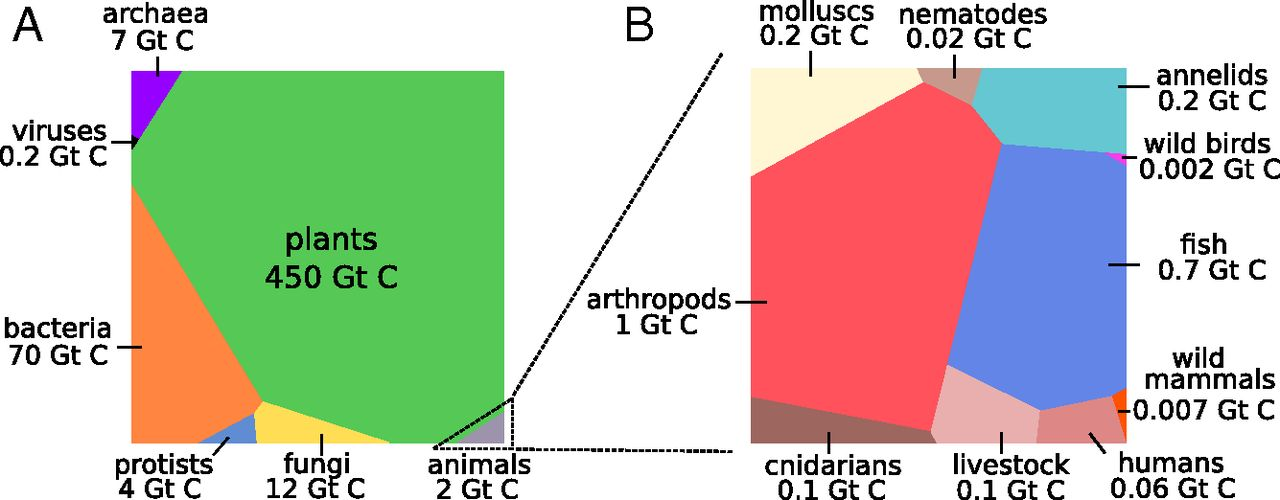
\includegraphics{figs/molbiol/biomass.jpeg}
  \caption[][6pt]{Distribution of biomass by taxa. Plants make up the majority of biomass on Earth, followed by bacteria and animals. Humans make up less than 0.01\% of the total biomass. The figure is from ``The biomass distribution on Earth'' by Bar-On, Phillips, and Milo (2018), published in the journal {\em Proceedings of the National Academy of Sciences} (PNAS), where they estimate the total biomass of Earth to be around 550 gigatons of carbon, with 80\% of this biomass composed of plants, 13\% of bacteria, and only 0.01\% attributed to humans. Most of the animal biomass is composed of arthropods and fish.}
  \label{fig:biomass}
% https://en.wikipedia.org/wiki/Cellular_compartment
\end{figure}

Oh, did we mention taxa? We did. Like computer scientists, biologists like to organize and classify entities of their study into groups and hierarchies. Taxonomy is the science of classifying living things into groups based on common characteristics. The basic unit of taxonomy is the species, which is a group of organisms that can interbreed and produce fertile offspring. Species are further grouped into genera, families, orders, classes, phyla, and kingdoms. The highest level of classification is the domain, which is based on molecular data and includes three groups: Bacteria, Archaea, and Eukarya. These domains are based on differences in the genetic material of organisms and reflect the evolutionary relationships between them.

\begin{figure}
  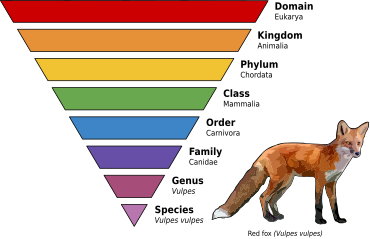
\includegraphics[width=0.8\textwidth]{figs/molbiol/taxonomy.png}
  \caption[][6pt]{Major ranks in biological taxonomy: from species at the bottom to domains at the top. Also shown is the naming of the red fox, \textit{Vulpes vulpes}. All living organisms are named according to their genus and species, and since these names are in Latin, they are italicised. The first letter of the genus is capitalised and the species name is lower case. Often biologists would shorten this naming by using the first letter of the genus and the full species name, as in the example of the red fox, \textit{V. vulpes}.}
  \label{fig:taxonomy}
% https://en.wikipedia.org/wiki/Cellular_compartment
\end{figure}


\section{Properties of Life}

Let's start by considering what defines something as living. Today we know that there are many types of organisms, including animals, plants, fungi, and microorganisms. Despite their differences, all living organisms share certain characteristics not found in non-living things. These characteristics of life include being composed of cells -- the basic units of life -- the ability to grow and develop, to reproduce, to respond to stimuli, and to maintain internal balance, like humans who maintain their body temperature at \(37^\circ\mathrm{C}\). All of these functions require energy, which living organisms obtain by consuming food or other organisms. The ability to evolve and adapt to changing environments is another key characteristic of life. This is why we have so many different species on Earth, each adapted to its own niche.

\section{The Cell}

Cells are the Basic Units of Life
\reversemarginpar
\marginnote{The estimate of the number of cells in the human body comes from the study ``An estimation of the number of cells in the human body'' published by Bianconi et al. in the {\em Annals of Human Biology} (2013), which provides a comprehensive calculation of the number of cells in different tissues. The number is approximate, as it can vary depending on individual factors such as size and health.}
\normalmarginpar
All living organisms consist of one or more cells. Cells are the building blocks of life and are responsible for carrying out the processes that sustain life. They are highly organized structures that contain all the necessary components to carry out the functions of life. 

Some organisms consist of a single cell, and we refer to them as single-celled organisms. Examples of single-celled organisms include bacteria, archaea, and protists. These organisms are capable of performing all the functions of life within a single cell. Single-celled organisms are the most abundant form of life on Earth and are found in almost every environment, from the deep sea to the soil to the human gut. They are of particular interest to biologists because a single cell can be easier to study than a complex organism with many cells. 

Single-celled organisms are classified as either prokaryotes or eukaryotes. Prokaryotes are single-celled organisms that lack a defined nucleus or other membrane-bound organelles. They include bacteria and archaea. Eukaryotes are organisms that have a defined nucleus and membrane-bound organelles. Examples of unicellular eukaryotes include certain types of algae, protozoa, and fungi such as yeast. (More on the nucleus later.)

Multicellular organisms are made up of many cells that work together. Humans, for example, are made up of \(6 \times 10^{13}\) cells. That's 60 trillion cells, or
$$ 60,000,000,000,000 {\ \rm cells}. $$
For comparison, there are about 300 billion stars in the Milky Way, so we have about 200 times more cells in our bodies than there are stars.

Molecular biologists used to define cell types based on how they looked under the microscope, but now we can also define them based on their molecular characteristics, such as the genes they express. There is a special field of molecular biology called single-cell transcriptomics, which studies the gene expression of individual cells. This field has revolutionized our understanding of cell types and their functions. More about this later in the course.

Figure~\ref{fig:cell} shows a diagram of a typical eukaryotic cell. Is it an animal or plant cell? What organelles can you identify? The cell is a complex structure with many different parts, each with a specific function. Some of the most important organelles in a eukaryotic cell are the nucleus, which contains the genetic material, the mitochondria, which produce the cell's energy, and the endoplasmic reticulum, which is involved in protein synthesis. Plant cells have some additional organelles, such as chloroplasts, which are involved in photosynthesis, and a large central vacuole, which stores water and nutrients.

\begin{figure}[h!]
    \centering{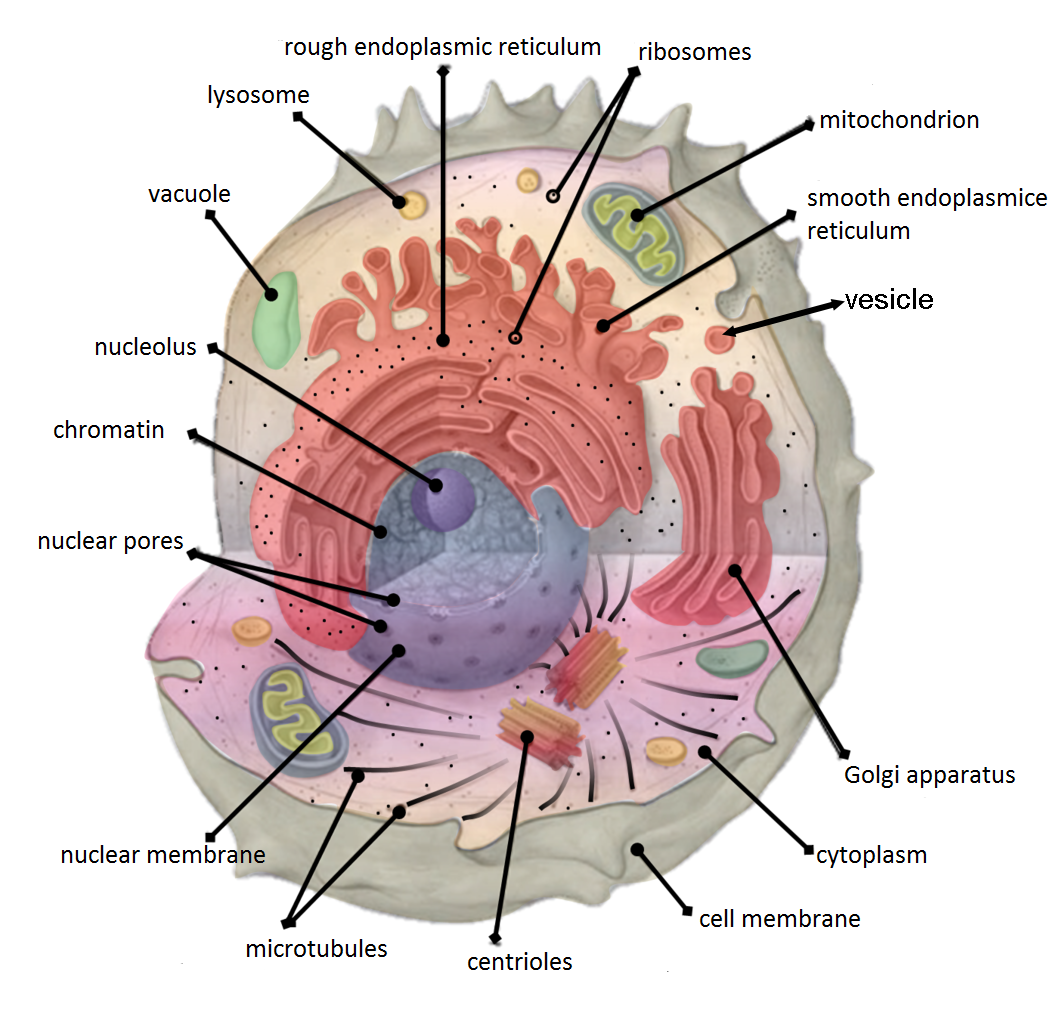
\includegraphics[width=0.8\textwidth]{figs/molbiol/cell.png}}
    \caption[][6pt]{The model of a eukaryotic cell, with some of its organelles labeled. Note that this is only a model, and that the actual cell is much more complex.}
    \label{fig:cell}
% https://en.wikipedia.org/wiki/Cellular_compartment
\end{figure}

\section{Cells Die and Are Replaced}

Cells in the human body are constantly dying and being replaced. Approximately 96 million cells die every minute as part of the natural process of cell turnover. The lifespan of a cell varies greatly depending on its type. For example, white blood cells typically survive for about 13 days, while epidermal skin cells last about a month. Red blood cells, which carry oxygen, have a lifespan of about 120 days. Liver cells, which are involved in vital metabolic processes, can live for about a year and a half before they are replaced. This continuous cycle of cell death and regeneration is essential for maintaining the health and function of the body.


\section{What Makes Up the Cell?}

A cell is made up of many components, but primarily water (about 70\%) and proteins (about 20\%). Water serves as the cell's medium, providing an environment in which biochemical reactions can take place. Proteins are large biomolecules, typically made up of thousands or more atoms, that play critical roles in the cell, acting as building blocks, catalyzing chemical reactions, and forming membranes.

The remaining 10\% of the cell is made up of smaller molecules, including sugars, fatty acids, signaling molecules, and energy-related molecules. If these smaller molecules were left alone, nothing significant would happen. It is the proteins that drive all essential cellular processes. They are the true engines of the cell, making everything inside the cell happen, and ultimately sustaining life.

\section{Proteins}

Proteins are large, complex molecules that are essential to life and are involved in almost every cellular process, from building and repairing tissues to regulating metabolism and transmitting signals. They are the workhorses of the cell, carrying out the functions that sustain life.

Proteins are made up of long chains of amino acids linked together in a specific sequence. All organisms, with a few exceptions, use 20 amino acids that can be combined in various ways to produce diverse proteins. The sequence of amino acids in a protein determines its structure and function. Proteins range in size from 50 to 30,000 amino acids, with the average human protein containing about 300.

Proteins have a complex three-dimensional structure that is critical to their function. A protein's structure is determined by its amino acid sequence and the interactions between the amino acids. Proteins can fold into specific shapes that allow them to interact with other molecules in the cell. Protein structure is described at four levels: primary (the amino acid sequence), secondary (local folding into helices or sheets), tertiary (the overall three-dimensional shape), and quaternary (the arrangement of multiple subunits into a larger complex).

For example, human insulin consists of 51 amino acids. The image in Fig.~\ref{fig:insulin-secondary} shows the secondary structure of human insulin. The primary structure of a protein is a sequence of amino acids that make up the molecule. In this figure, the amino acids are marked with circles containing a three-letter abbreviation. For example, the insulin chain begins with Met, which is an abbreviation for methionine. The secondary structure of a protein refers to local folding patterns, such as helices and sheets, which are important because they determine how the protein will fold into its three-dimensional shape.

\begin{figure}
    \centering{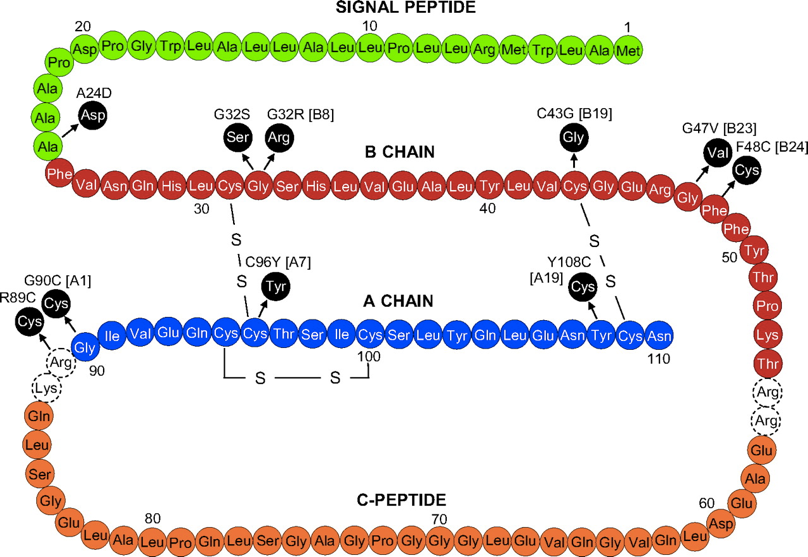
\includegraphics[width=0.9\textwidth]{figs/molbiol/insulin-chain.png}}
    \caption[][6pt]{Primary structure of insulin.}
    \label{fig:insulin-secondary}
\end{figure}

The folding of a protein defines its function. Its tertiary structure gives the actual three-dimensional structure of the protein. Fig.~\ref{fig:insulin-3d} is what insulin looks like in 3D, where the representation of the amino acid sequences has been abstracted with parts represented as sheets and helices (don't worry about them now).

\begin{figure}
    \centering{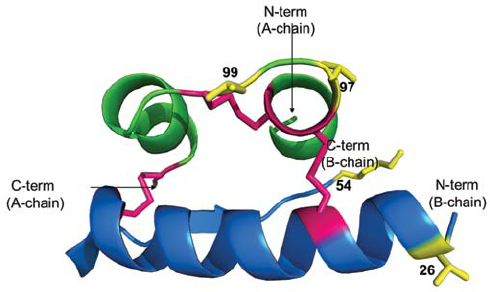
\includegraphics[width=0.7\textwidth]{figs/molbiol/insulin-3d.png}}
    \caption[][6pt]{Tertiary structure of an insulin.}
    \label{fig:insulin-3d}
\end{figure}

A protein's structure is critical to its function, as proteins fold into complex three-dimensional shapes that allow them to interact with other molecules in the cell. A protein’s shape, determined by its amino acid sequence and interactions, can also change in response to cellular signals to perform specific functions.

Another example is leptin (Figure~\ref{fig:leptin}). Leptin is a hormone that helps regulate energy balance by inhibiting hunger. It is composed of 167 amino acids, and its tertiary structure is shown below. A deficiency of leptin leads to obesity. Molecular biologists have studied this in several model organisms, including mice.

\begin{figure}
    \centering{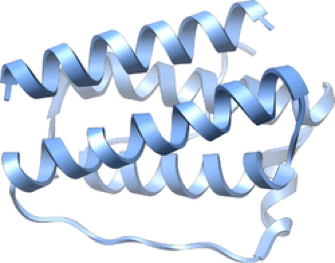
\includegraphics[width=0.6\textwidth]{figs/molbiol/leptin.png}}
    \caption[][6pt]{Tertiary structure of a leptin.}
    \label{fig:leptin}
\end{figure}

The three-dimensional structures of proteins are often quite amazing. Consider chaperonins, a class of proteins that provide favorable conditions for the proper folding of other proteins. Fig.~\ref{fig:chaperonin} shows a rendering of their structure. Chaperonins form a protective chamber that allows proteins to fold correctly without interference from other molecules. Chaperonins are found in all cells and are critical for maintaining the health and function of the cell.
    
\begin{figure}
    \centering{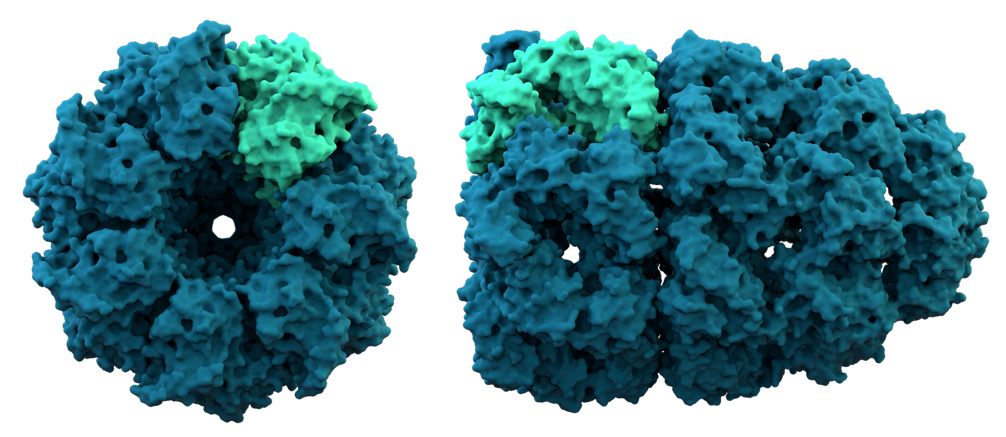
\includegraphics[width=0.8\textwidth]{figs/molbiol/chaperonin.png}}
    \caption[][6pt]{Tertiary structure of a chaperonin.}
    \label{fig:chaperonin}
\end{figure}

\section{Amino Acids}

We have talked about amino acid chains, but we have never really said what they are. Now is the time. An amino acid is a simple organic compound containing both a carboxylic acid (-COOH), an amino group (-NH2), and a variable side chain (labeled R). Fig.~\ref{fig:aminoacid} shows the chemical structure of an amino acid.

\begin{marginfigure}
    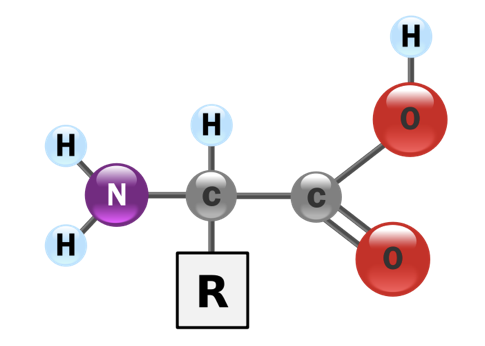
\includegraphics{figs/molbiol/aminoacid.png}
    \caption[6pt]{Chemical structure of an amino acid.}
    \label{fig:aminoacid}
\end{marginfigure}

The side chain is what defines each amino acid. Around 500 amino acids are known, but only twenty are commonly found in living organisms. It's worth noting that there are exceptions, as biology often defies strict rules, but this isn't the time to dive into those details. Some side chains are very simple; for example, the side chain of glycine is just a single hydrogen atom. Fig.~\ref{fig:aminoacids} shows all twenty side chains and the corresponding names of their amino acids.

\begin{figure}
    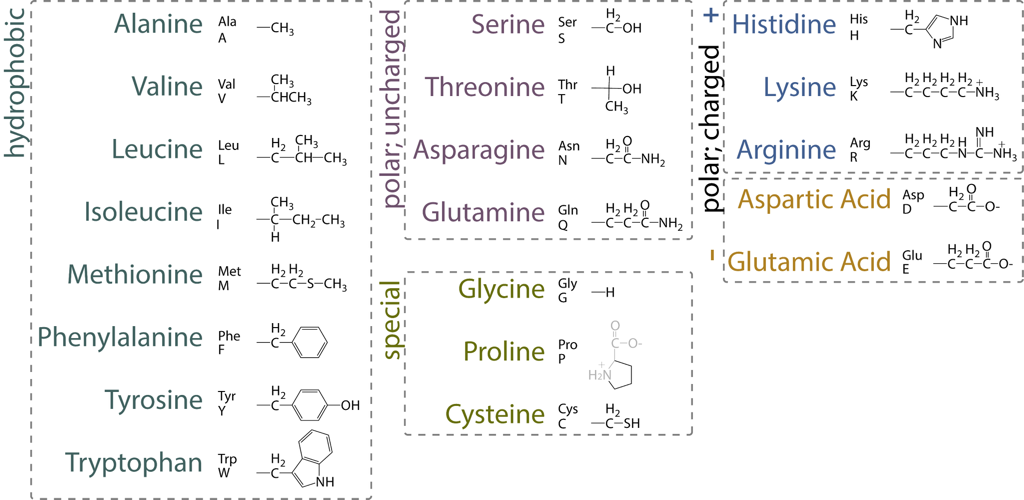
\includegraphics{figs/molbiol/aminoacids.png}
    \caption[6pt]{Chemical structure of an amino acid.}
    \label{fig:aminoacids}
\end{figure}

Proteins are chains of amino acids. They are actually made by linking amino acids together, in a row, one by one. The process is called polymerization, a condensation reaction in which two amino acids are linked by a peptide bond between the carbon of one and the nitrogen of the other. Here is a graphical depiction of the process. Fig.~\ref{fig:peptide-bond} shows the reaction that forms a peptide bond between two amino acids. The amino acids are shown in their abbreviated form, with the side chain represented by the letter R. The peptide bond is formed between the carboxyl group of one amino acid and the amino group of the other amino acid. The resulting molecule is called a dipeptide.

\begin{figure}
    \centering{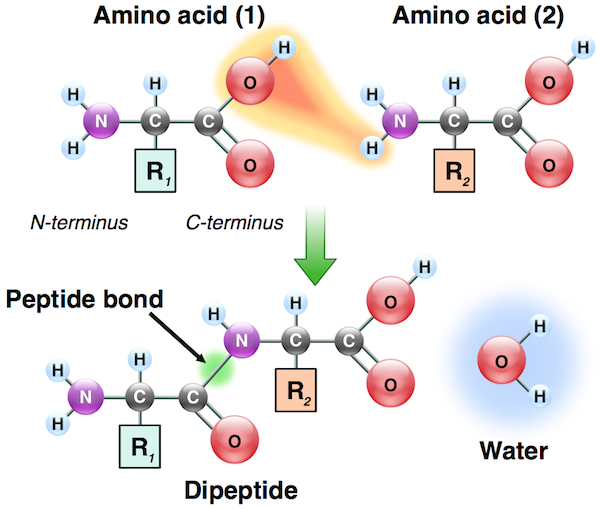
\includegraphics[width=0.65\textwidth]{figs/molbiol/peptide-bond.png}}
    \caption[6pt]{Formation of a peptide bond between two amino acids.}
    \label{fig:peptide-bond}
\end{figure}

The process of polymerization continues until the protein is complete, producing a chain of amino acids called a polypeptide. This chain then folds into a specific three-dimensional shape, determined by the amino acid sequence, cellular environment, and interactions among amino acids, and this folding defines the protein’s function.

\section{Metabolism}

Metabolism is the set of chemical reactions that occur in living organisms to maintain life. These reactions are essential for the growth, development, and reproduction of organisms. Metabolism can be divided into two main categories: catabolism and anabolism. Catabolism refers to the breakdown of complex molecules into simpler ones, releasing energy in the process. Anabolism refers to the synthesis of complex molecules from simpler ones, requiring energy. Together, these processes balance cellular energy and enable the cell to function.

Metabolism is regulated by enzymes, which are proteins that catalyze chemical reactions in the cell. Enzymes are highly specific, each catalyzing only one reaction. They can speed up reactions by a factor of up to a billion times.

Here is an example of a metabolic pathway: glycolysis. Glycolysis is the breakdown of glucose into pyruvate, a process that releases energy. As shown in Fig.~\ref{fig:glycolysis}, glycolysis is the first step in cellular respiration, which generates energy for the cell. The energy released is used to produce ATP, the cell's primary energy source.

\begin{figure*}
    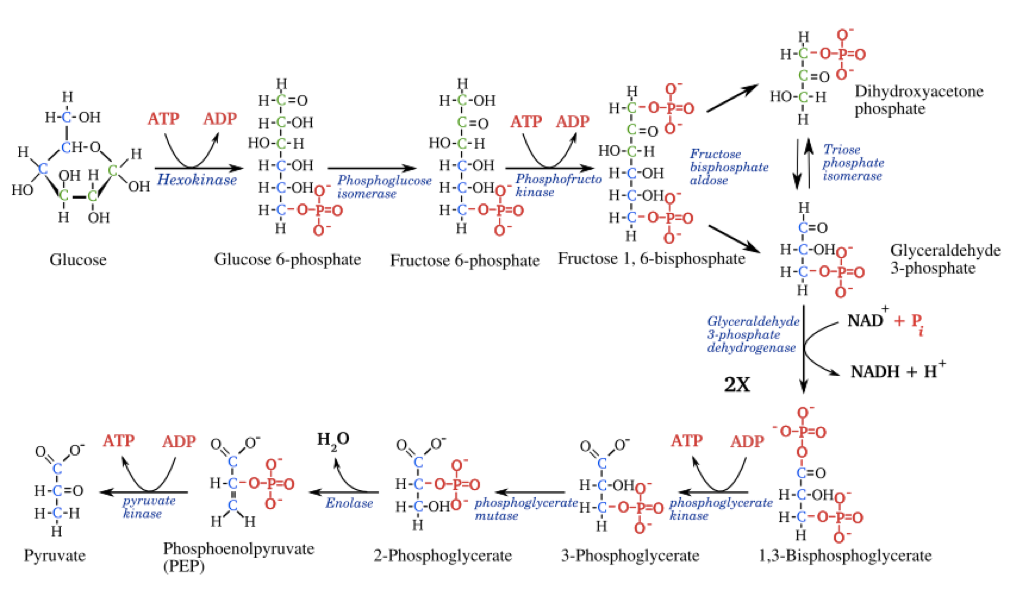
\includegraphics{figs/molbiol/glycolysis.png}
    \caption[6pt]{The glycolysis pathway.}
    \label{fig:glycolysis}
\end{figure*}

Chemicals such as glucose, fructose 6-phosphate, and others that serve as entry points, final products, or intermediates in chemical reactions are called metabolites. Glycolysis is an example of a metabolic pathway. All the reactions in glycolysis are catalyzed by enzymes, which are proteins that catalyze reactions that would otherwise occur too slowly to sustain life. Proteins in this and other pathways often have complex names that can be difficult for computer scientists to remember. For example, the enzyme that converts glucose 6-phosphate to fructose 6-phosphate is called phosphofructokinase. Fortunately, we don't need to memorize these names, but it's crucial to understand that almost no reaction in living organisms would happen without proteins. Proteins are essential to metabolic pathways and are key to making cells function and stay alive.

Just for a taste, Fig.~\ref{fig:glycolysis} shows what hexokinase looks like (find it in the glycolysis pathway--what does it do?). It consists of 617 amino acids.

\begin{figure}
    \centering{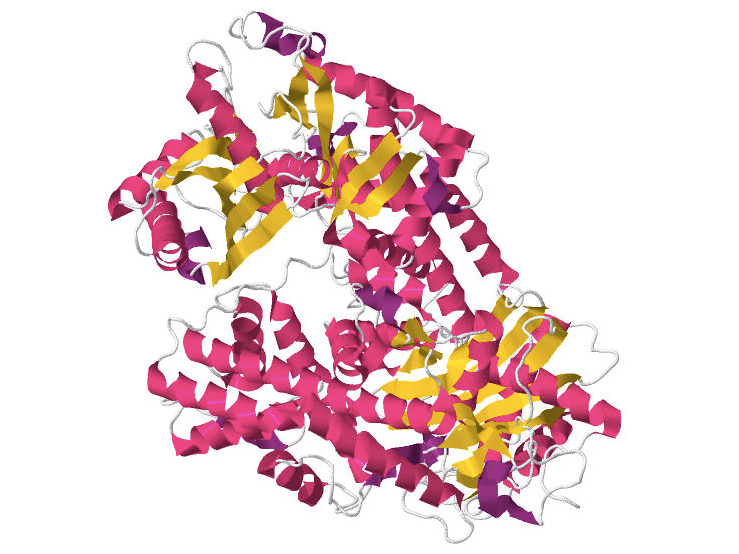
\includegraphics[width=0.7\textwidth]{figs/molbiol/hexokinase.png}}
    \caption[][6pt]{Tertiary structure of a hexokinase.}
    \label{fig:hexokinase}
\end{figure}

\section{Some More Surprising Facts}

A typical protein is about 5 nm in size, while a typical eukaryotic cell is around 50 µm. The diameter of a cell is approximately 10,000 times larger than that of an average protein. Since volume scales with the cube of the diameter, the volume of the cell is roughly $10,000^3 = 10^{12}$ times larger than the volume of a typical protein.

Incredibly, each cell contains around one billion protein molecules ($10^9$). This astonishing number highlights the immense molecular complexity of even a single cell.

To add more perspective, there are about two million different protein types in the human body. The longest known protein, titin, consists of about 27,000 amino acids.

\section{Proteins Degrade}

Ok, so we have quite a lot of proteins in each cell. They are present, do their work, and then just stay there, unchanged. This idea seems to fit with what we learned in high school biology, where we were told that enzymes are not consumed in the reactions they catalyze. So, does that mean enzymes--and proteins in general--just stay in the cell forever?

Not quite. Proteins have a limited lifespan—they do not last forever. They are continually degraded, often within hours. Here's the abstract of the publication where they have measured degradation rates (half-lives) for rat enzymes\marginnote{The publication is ``Degradation of glucose-metabolizing enzymes in the rat small intestine during starvation'' by G M Jones and R J Mayer, published in the {\em Biochemical Journal} (1973).}:

\begin{quote}
    \textit{1. The degradation rates and half-lives of hexokinase, 6-phosphogluconate dehydrogenase, lactate dehydrogenase, pyruvate kinase, glucose 6-phosphate dehydrogenase, phosphoglycerate kinase and aldolase were calculated from measurements of the decline in activities of these enzymes in rat small intestine during starvation. 2. The half-lives of the enzymes are: hexokinase, 5.7h; 6-phosphogluconate dehydrogenase, 7.6h; glucose 6-phosphate dehydrogenase, 6.0h; pyruvate kinase, 8.9h; lactate dehydrogenase, 8.7h; phosphoglycerate kinase, 8.7h; aldolase, 5.1h. 3. The significance of the results is discussed with respect to the regulation of enzyme concentrations in response to changes in diet.}
\end{quote}

\section{The Puzzle}

So now we know that cells contain vast numbers of proteins—and that proteins are what keep us alive. Yet they do not last very long, so someone has to make them. But who makes them, and where? Is there a separate factory for each of the two million different proteins, or a single factory that follows a recipe? And if so, where is that recipe stored?

\section{The Central Dogma of Molecular Biology}

The central dogma of molecular biology is a framework that describes the flow of genetic information in cells. It states that genetic information generally flows from DNA to RNA to protein. The central dogma is a fundamental principle of molecular biology and is essential for understanding how genetic information is stored, replicated, and expressed in living organisms.

In a nutshell, a discovery that took decades of research and earned numerous Nobel Prizes, the recipes for all the proteins involved in our lives are stored in a long molecule called DNA (Fig.~\ref{fig:dna-detail}), or deoxyribonucleic acid. In eukaryotes, DNA is tightly packed and stored in the nucleus of the cell. DNA is in the form of a double helix, with two complementary strands. Each strand is a chain of nucleotides attached to a sugar-phosphate backbone.

\begin{figure}
    \centering{\includegraphics[width=0.7\textwidth]{figs/molbiol/dna-detail.png}}
    \caption[6pt]{The structure of DNA.}
    \label{fig:dna-detail}
\end{figure}

There are only four different nucleotides: cytosine (C), guanine (G), adenine (A), and thymine (T). Across the strands, thymine forms hydrogen bonds with adenine, and cytosine with guanine (Fig.~\ref{fig:tacg-bonds}). The strands are therefore complementary and carry the same genetic information in complementary form.

\begin{figure}
    \centering{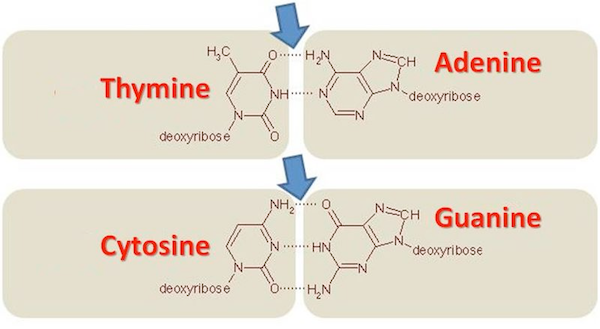
\includegraphics[width=0.8\textwidth]{figs/molbiol/tacg-bonds.png}}
    \caption[6pt]{Hydrogen bonds between nucleotides in DNA.}
    \label{fig:tacg-bonds}
\end{figure}

Did we say information? So soon! We were not there yet. But let us hurry (Fig.~\ref{fig:central-dogma}): Proteins are made in the cytoplasm, in factories called ribosomes. DNA—or rather a small subsequence of it—contains the recipe for a protein. This recipe must first be copied in the nucleus and then delivered to the ribosome. The carrier molecule is called RNA, ribonucleic acid. To conserve energy and avoid unnecessary complexity, Mother Nature figured out that it would be best to copy only the part of the DNA that encodes the amino acid sequence onto the RNA. This copying process is called transcription. The RNA (called messenger RNA because of its function) then travels from the nucleus to the ribosome, where its nucleotide sequence is translated into a sequence of amino acids, forming a protein.

\begin{figure}
    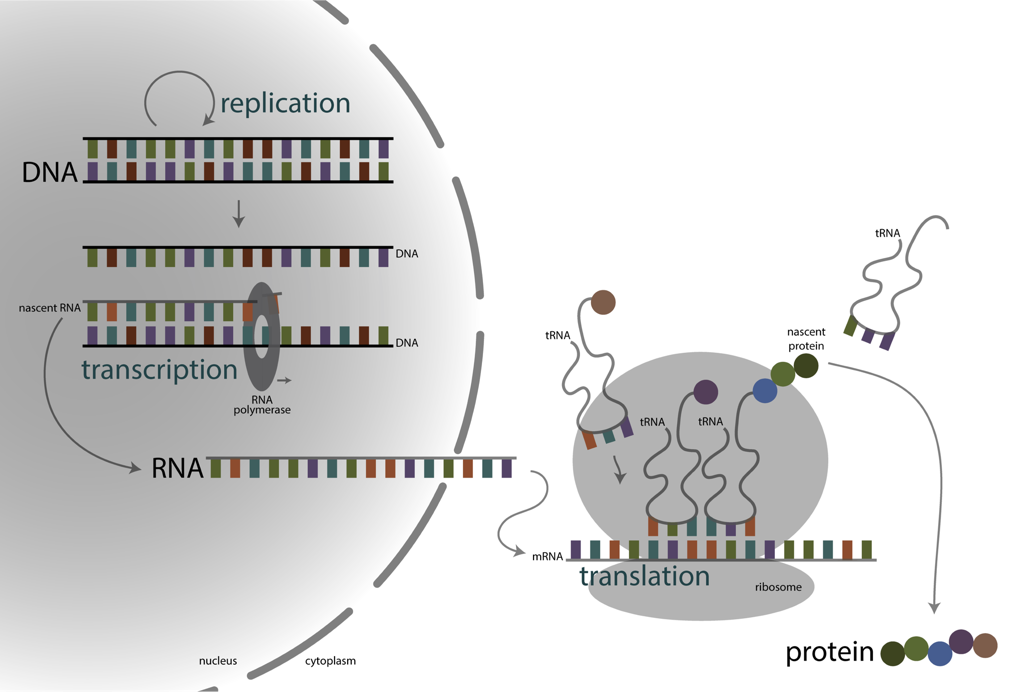
\includegraphics{figs/molbiol/central-dogma.png}
    \caption[][6pt]{The central dogma of molecular biology.}
    \label{fig:central-dogma}
\end{figure}

There are twenty amino acids that we need to encode. The encoding language consists of an alphabet of four nucleotides. A single letter from this alphabet is not sufficient to represent one of twenty amino acids, so we need words. Say that the length of the word is constant (we admit this may seem odd, but it is the simplest solution, and in the light of Occam's razor this assumption is perfectly acceptable). If we had words made of two nucleotides, they would encode $4 \times 4 = 16$ amino acids—not enough, since we need twenty. So we need at least three-letter words, or a sequence of three nucleotides. And, through evolution, a language with three-letter words emerged, each word encoding one amino acid. Different words encode the same amino acid, since there are $4 \times 4 \times 4 = 64$ possible combinations with a three-nucleotide sequence.

\begin{figure}
    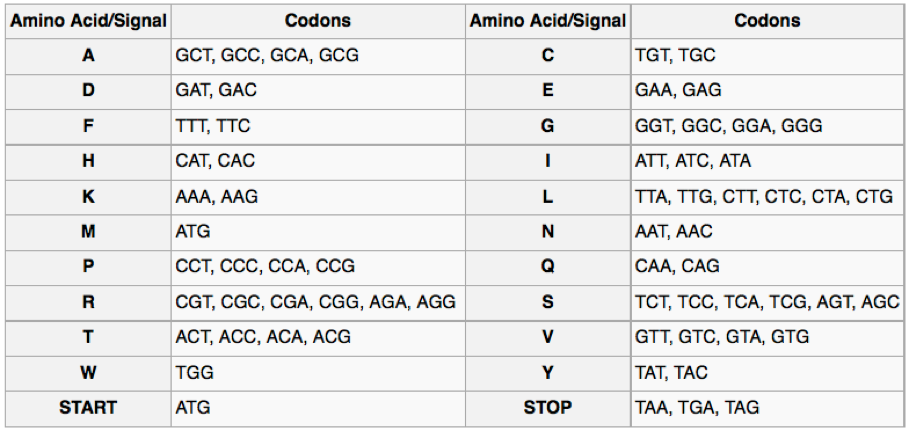
\includegraphics{figs/molbiol/code-of-life.png}
    \caption[][6pt]{The genetic code.}
    \label{fig:code-of-life}
\end{figure}

The sequence of three nucleotides is called a codon, the basic unit of the genetic code. The genetic code is the set of rules that determines how the nucleotide sequence of a gene is translated into the amino acid sequence of a protein. It is nearly universal, with the same codons encoding the same amino acids in almost all living organisms. It is also redundant, since most amino acids are encoded by more than one codon, and non-overlapping, meaning that each nucleotide is part of only one codon.

\section{What's Next?}

This is the beginning of molecular biology. But there are many open questions at this point. Here are just a few. For example, where are the parts of the DNA that contain the coding information for the proteins? How does transcription know where to find them? How many are there in all of DNA? How long is DNA, and how many nucleotides does it contain? Is there any other information stored in DNA? Are all proteins being made all the time? If not, who regulates this process, and how? Enough for this chapter. We should leave something for the rest of the course.
\chapter{A Brief History of \newline Central Dogma of Molecular Biology}

The central dogma of molecular biology is a key idea that explains how genetic information is used in living organisms. Proposed by Francis Crick in 1958, it describes the flow of information from DNA to RNA, and then to proteins, which perform most of the vital functions in cells. This concept has been foundational to the field of molecular biology and continues to shape our understanding of genetics.

\begin{marginfigure}
    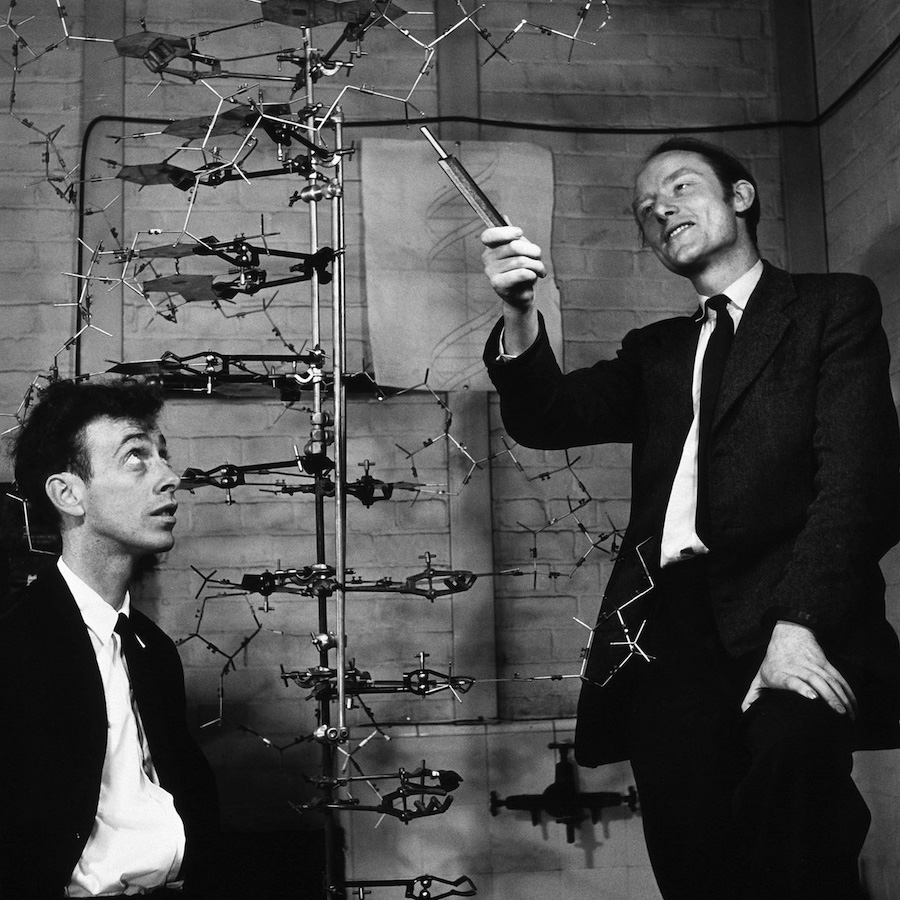
\includegraphics{figs/history/watson-crick-dna.jpeg}
    \caption[6pt]{Francis Crick and James Watson with their famous model of DNA.}
    \label{fig:watson-crick-dna}
\end{marginfigure}

Here are som of the major milestones, and some of accompanying stories, in the development of the central dogma of molecular biology:

\medskip\noindent\textbf{1953:} The double-helix structure of DNA was uncovered by James Watson, Francis Crick, and Rosalind Franklin. Franklin’s X-ray diffraction work was crucial in understanding the structure of DNA, although her contribution was underappreciated at the time. Without her clear images, the puzzle of DNA’s structure might have remained unsolved for much longer.

\begin{marginfigure}
    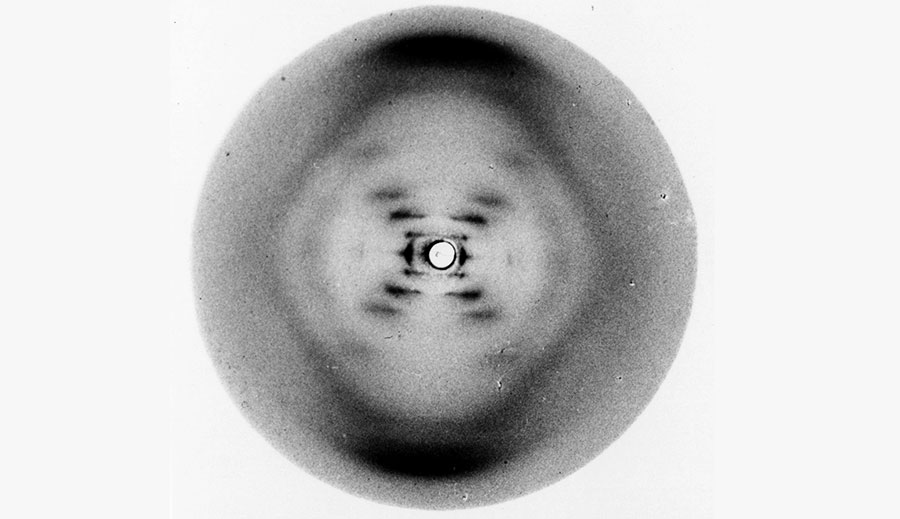
\includegraphics{figs/history/photograph-51.jpeg}
    \caption[6pt]{Photograph 51, the X-ray diffraction image of DNA taken by Rosalind Franklin.}
    \label{fig:photograph-51}
\end{marginfigure}

James Watson and Francis Crick's famous paper, titled "Molecular Structure of Nucleic Acids: A Structure for Deoxyribose Nucleic Acid," was published on April 25, 1953 in the journal Nature. This landmark paper was only about one page long but had a profound impact on biology, as it described the double-helix structure of DNA for the first time.

Towards the end of Watson and Crick’s 1953 paper, there is a famous sentence that reads:
\begin{quote}
    \textit{It has not escaped our notice that the specific pairing we have postulated immediately suggests a possible copying mechanism for the genetic material.}
\end{quote}
This sentence is understated yet profound. In a single line, Watson and Crick hint at one of the most important implications of their discovery: the double-helix structure of DNA naturally explains how genetic information can be copied during cell division. The specific pairing between the nucleotide bases (adenine with thymine, and guanine with cytosine) suggested a mechanism by which each strand of the DNA molecule could serve as a template for creating a new, complementary strand. This was a subtle but powerful insight, as it laid the foundation for understanding DNA replication—a central process in biology that ensures genetic continuity from one generation to the next. The modest tone of the sentence belied its transformative impact on genetics and molecular biology.

Notice that the discovery of the structure of DNA was hard and not without faults, even by the most influential scientists of the time. Linus Pauling, one of the most renowned chemists of the era, proposed a triple-helix model for DNA in 1953, placing the phosphate backbone in the center and the nucleotide bases on the outside. This model was fundamentally flawed due to charge repulsion between phosphate groups and its failure to account for base pairing. Pauling’s proposal, though influential, did not align with emerging experimental data, which ultimately led to the correct double-helix structure by Watson and Crick.

\begin{marginfigure}
    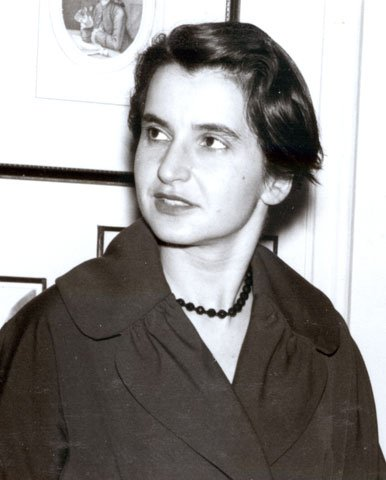
\includegraphics{figs/history/rosalind-franklin.jpeg}
    \caption[6pt]{Rosalind Franklin.}
    \label{fig:franklin}
\end{marginfigure}

\medskip\noindent\textbf{1958:} Francis Crick introduced the central dogma, explaining that information flows in one direction: from DNA to RNA to proteins. Proteins are the molecules that perform most functions within a cell, and they are produced according to instructions stored in DNA.

\medskip\noindent\textbf{1961:} François Jacob and Jacques Monod discovered messenger RNA (mRNA), which showed that RNA carries instructions from DNA to the cell's protein factories. This helped confirm that RNA acts as a temporary messenger in the process of turning genetic information into proteins.

\medskip\noindent\textbf{1966:} The cracking of the genetic code was a major scientific breakthrough. A group of scientists, including \textit{Marshall Nirenberg}, \textit{Har Gobind Khorana}, and members of the \textit{RNA Tie Club}, worked tirelessly to decipher how sequences of RNA are translated into amino acids, which are the building blocks of proteins. The \textit{RNA Tie Club} was an informal but competitive group of 20 scientists, each member representing one of the 20 amino acids. They wore black silk ties emblazoned with the symbol for RNA. Despite the serious goal of cracking the genetic code, there was a sense of humor and camaraderie in the group.

An anecdote is that they created their own membership pins and made grand declarations, like ``each amino acid will be solved by a club member!'' However, the race to crack the code was so competitive that, in the end, the discoveries were made by a few scientists outside the club. Still, the members’ friendly competition and idea-sharing helped push the field forward.

\bigskip\noindent\textbf{1970:} Howard Temin and David Baltimore discovered reverse transcriptase, an enzyme that allows RNA to be copied back into DNA. This discovery overturned the assumption that the flow of genetic information was strictly one-way and provided crucial insights into how retroviruses like HIV function.

\bigskip\noindent
For computer scientists, the central dogma provides a blueprint for how biological data is organized. DNA is the database, RNA acts as a dynamic intermediary, and proteins are the functional outcomes. In bioinformatics, understanding these relationships is key to analyzing genetic sequences, predicting protein structures, and exploring the effects of mutations.
\chapter{Genomes and Some Simple Sequence Patterns}
\label{ch:genome}

The central dogma of molecular biology (Fig.~\ref{fig:g-central-dogma-genome}), as we have already discussed in Chapter~\ref{ch:intro-mol-biol}, explains how genetic information flows within living systems. In simple terms, it states that "DNA makes RNA makes protein." To elaborate, DNA contains the instructions for the sequence of amino acids in proteins. To create a protein, the information from the DNA—known as the protein-coding sequence—is first transcribed into messenger RNA (mRNA) and then translated into a protein. The central dogma also emphasizes that this is the only direction in which information flows: the sequence of amino acids in proteins cannot be converted back into DNA.

\begin{figure}
  \centering{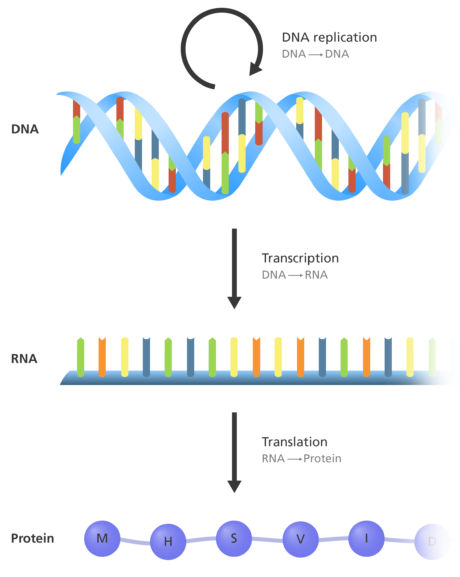
\includegraphics[width=0.5\textwidth]{figs/genome/central-dogma.png}}
  \caption[6pt]{The central dogma of molecular biology.}
  \label{fig:g-central-dogma-genome}
\end{figure}

At this stage, however, we should mention that biology is full of exceptions and surprises. The central dogma is a fundamental principle of molecular biology, but it is not the only way in which genetic information is used in living systems. For example, some RNA molecules possess catalytic activity, and some proteins bind to DNA to regulate gene expression. In addition, the central dogma does not account for the many ways in which genetic information can be modified, such as through mutations, recombination, or epigenetic changes. Nevertheless, the central dogma provides a useful framework for understanding how genetic information is stored, transmitted, and used in living systems.

In this chapter, we will begin to explore genomes and DNA sequences.
\marginnote{Even in stretches of DNA once thought to be “junk,” researchers have found recurring motifs and structural patterns — hints that randomness in the genome is often an illusion.}
Our goal is to investigate whether these sequences are simply random arrangements of nucleotides or if there are recognizable patterns that can be identified, even without considering genes. Understanding these patterns can provide valuable insights into the structure and function of DNA. We will focus on genes in the next chapter, where we will delve deeper into their roles and significance.

\section{Structure of Deoxyribonucleic Acid (DNA)}

Deoxyribonucleic acid (DNA) is a long molecule composed of nucleotides, which consist of a sugar called deoxyribose, a phosphate group, and a nitrogenous base~(Fig.~\ref{fig:g-dna-detail}). There are four types of nucleotides: cytosine (C), guanine (G), adenine (A), and thymine (T). DNA consists of two strands that twist around each other to form a double helix. The strands are held together by weak hydrogen bonds, with adenine pairing with thymine and cytosine pairing with guanine.

\begin{figure}
    \centering{
        \includegraphics[width=0.6\textwidth]{figs/genome/dna-detail.png}
    }
    \caption[6pt]{The structure of DNA.}
    \label{fig:g-dna-detail}
  \end{figure}

  Each strand has a repeating pattern of deoxyribose sugars and phosphates, forming a strong sugar-phosphate backbone. The nucleotides are attached to this backbone, with one nucleotide connected to each sugar molecule.

Because the two strands are complementary, one strand can always be used to determine the sequence of the other. Both strands carry the same genetic information, which is crucial for accurate DNA replication.

The difference in bond strength gives DNA a zipper-like quality. The weak hydrogen bonds make it easy to unzip the strands, while the strong covalent bonds in the backbone protect the structure from damage. This design provides both flexibility and stability, allowing DNA to perform its role effectively in biological systems.

\section{Directionality of DNA Strands}

The two strands of DNA run in opposite directions, a property known as antiparallel orientation\marginnote{The antiparallel discovery was crucial for understanding DNA replication — it was one of the insights that helped Watson and Crick correctly model the double helix in 1953.}. To understand this concept, we need to examine the sugar group in the sugar-phosphate backbone. Chemists have established a system for numbering the carbon atoms in the sugar molecule, labeling them with ``prime'' notation, such as 1' (one-prime), 3' (three-prime), and so on. This notation helps organize the chemical structure and provides a clear reference for the orientation of the strands. Figure~\ref{fig:g-sugar} illustrates the atom numbering for the sugar group.

\begin{marginfigure}
  \centering{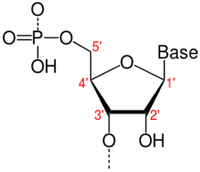
\includegraphics{figs/genome/sugar.png}}
  \caption[6pt]{Numbering of carbon atoms in a sugar group.}
  \label{fig:g-sugar}
\end{marginfigure}

In the DNA backbone, each sugar is linked to a phosphate group at its 5'-end (five-prime end) and to the next nucleotide through its 3'-end (three-prime end). The 5'-end of a DNA strand refers to the end with a free phosphate group attached to the 5' carbon of the sugar, while the 3'-end refers to the end with a free hydroxyl group (-OH) attached to the 3' carbon of the sugar.

This arrangement gives each DNA strand its own directionality. One strand runs from the 5' end to the 3' end, while the complementary strand runs in the opposite direction, from 3' to 5'. This antiparallel structure is critical for many biological processes, such as DNA replication and transcription. The enzymes involved in these processes recognize the direction of each strand and ensure that the genetic information is copied or read correctly.

The 5' to 3' orientation also plays an essential role in the regulation of gene expression, as this directionality influences how various molecules interact with DNA during cellular processes. Understanding this fundamental concept is crucial to grasping the mechanisms that underlie molecular biology and the flow of genetic information.

\section{Genome Size and Packaging}

The complete DNA sequence of an organism is called its genome. The genome represents the total genetic information contained within a cell, including the DNA in the nucleus and within any organelles. Interestingly, some organelles also contain their own DNA
\marginnote{Mitochondria and chloroplasts likely originated from ancient bacteria that formed symbiotic relationships with early eukaryotic cells—a concept known as the \textit{endosymbiotic theory}.}. In animals, this organelle is the mitochondrion, and in plants, it is the chloroplast. However, when we refer to the genome of a eukaryote, we usually mean the DNA in the nucleus. The genetic material in the mitochondria is referred to as the mitochondrial DNA (mtDNA) or mitochondrial genome.

In the nucleus, DNA is typically not a single continuous molecule but is instead divided into segments and organized into chromosomes. For example, humans have 23 pairs of chromosomes. However, we won't focus on chromosomes for now, so there's no need to worry about them in the next few lectures.

This structure allows the genome to be efficiently packaged and organized, facilitating processes such as cell division and gene expression. The size of the genome can vary greatly between species, but it always contains all the information necessary for the development, function, and reproduction of the organism.

So, what is the total length of the DNA sequence? It depends on the organism, as shown in Figure~\ref{fig:g-genome-size}. Prokaryotes, such as bacteria, have the shortest genomes. We measure DNA length in base pairs (bp), which refer to two nucleobases bound together by hydrogen bonds. Simply put, one base pair consists of one nucleotide on each strand of the DNA. The total number of nucleotides on one strand determines the overall size (or length) of the genome.

\begin{figure}
    \centering{
        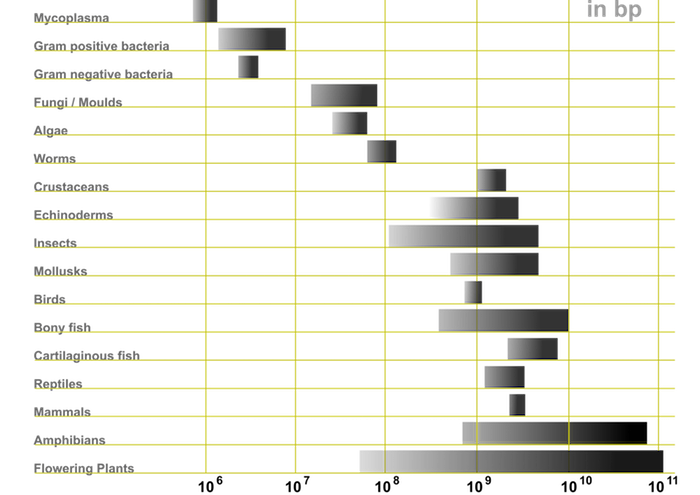
\includegraphics[width=0.95\textwidth]{figs/genome/genome-size.png}
    }
    \caption[6pt]{Genome sizes of various organisms.}
    \label{fig:g-genome-size}
  \end{figure}

Bacterial genomes typically range from 0.5 to 13 megabase pairs (Mbp), where one Mbp equals one million (10\textsuperscript{6}) base pairs. The abbreviation ``Mb'' is often used to represent megabases (megabase pairs). In prokaryotes, the genome is usually circular, while in eukaryotes it is typically linear and distributed among multiple chromosomes. This distinction has important implications for how DNA is replicated and organized within the cell.

Eukaryotic genomes are much larger\marginnote{Curiously, genome size does not correlate with organism complexity — an onion has far more DNA than a human. This puzzle is known as the \textit{C-value paradox}, reminding us that more DNA doesn’t necessarily mean a “more advanced” organism.}, ranging from 8 Mb to 670 gigabase pairs (Gb), with one Gb equaling one billion (10\textsuperscript{9}) base pairs. In contrast, viruses have much smaller genomes, ranging in size from 5 to 50 kilobase pairs (kb), where one kb equals one thousand (10\textsuperscript{3}) base pairs.

And what about us, humans? Our genome contains about 3,200 Mb (or 3.2 Gb). To put that in perspective, the first Harry Potter book, Harry Potter and the Philosopher’s Stone, contains approximately 76,944 words. With the average English word being just over five letters long, the book contains roughly 384,720 letters. If we represented each nucleotide in the human genome as a single letter, we would need the equivalent of about 8,300 copies of Philosopher’s Stone to write out the entire human genome. To visualize this further, a typical version of Harry Potter and the Philosopher’s Stone is about 2 cm thick. If we stacked 8,300 of these books, one on top of another, the stack would reach a height of around 166 meters.

If we could stretch out the DNA from a single human cell, it would form a very thin thread about 2 meters long. Despite this length, the DNA is tightly packed into the cell's nucleus, which is only about 5–10 micrometers in diameter. This incredible compaction is made possible because the DNA is wrapped around proteins called histones, forming a structure known as chromatin. This efficient organization allows the large amount of DNA to fit neatly inside the tiny space of the cell nucleus.

\section{Exploring Viral Genomes: Lambda Phage as a Case Study}

Let us start small—with a virus. The lambda phage\marginnote{The lambda phage has been a cornerstone of molecular biology since the 1950s—it helped scientists uncover how genes are regulated, leading to the discovery of genetic switches and laying groundwork for modern genetics.} is a bacterial virus that infects and destroys \textit{Escherichia coli} bacteria. This virus, like many others, has its genome fully sequenced and available for research. You may have noticed the scientific name \textit{Escherichia coli}. These names follow the rules of binomial nomenclature, a system that uses Latin names composed of a genus and species. For example, humans are classified as \textit{Homo sapiens}.

Now, back to the lambda phage. One of the sources for its genome information is GenBank\footnote{\url{https://www.ncbi.nlm.nih.gov/genbank}},
a sequence database maintained by the National Center for Biotechnology Information (NCBI). GenBank hosts a page dedicated to the lambda phage genome\footnote{\url{https://www.ncbi.nlm.nih.gov/nuccore/NC_001416.1}}.

The GenBank page
\marginnote{GenBank isn’t alone—similar databases include EMBL-EBI’s ENA in Europe and DDBJ in Japan. Together, these three form the International Nucleotide Sequence Database Collaboration, ensuring that every submitted sequence is synchronized and globally accessible.}
contains several key pieces of information.
It includes data about the scientists and research groups that sequenced and published the genome, as well as a detailed description of the genome’s structure. The page also lists the specific genes encoded within the genome and their functions. Finally, at the bottom of the page, you'll find the complete DNA sequence of the lambda phage, represented as a string of nucleotides (A, T, C, and G). This sequence is what we are most interested in for bioinformatics analyses. If you are curious about the meaning of the various fields and terms on GenBank's page, you can refer to the Sample GenBank Record page\footnote{\url{https://www.ncbi.nlm.nih.gov/genbank/samplerecord}}. Clicking on any of the terms will provide an explanation of their significance.

While all this information is available through the GenBank's web page, we are more focused on how to access it programmatically. This allows us to automate the retrieval of genomic data for further analysis and manipulation, which is essential for large-scale bioinformatics tasks. Programmatic access ensures reproducibility, scalability, and the ability to integrate data retrieval directly into analytical pipelines. 

In the following example, we will see how to retrieve the lambda phage genome sequence using Python:

\vspace*{3mm}
\begin{lstlisting}
>>> from Bio import Entrez, SeqIO
>>> Entrez.email = "blaz.zupan@fri.uni-lj.si"
>>> with Entrez.efetch(db="nucleotide", 
>>>   id="NC_001416", rettype="gb") as handle:
>>>    data = SeqIO.read(handle, "genbank")
>>> len(data.seq)
48502
>>> data.seq[:10]
Seq('GGGCGGCGAC')
\end{lstlisting}

The genome of {\em Lambda phage} contains 48,502 base pairs. We have the sequence for only one strand; the other strand is simply its reverse complement. The genome starts with three guanine nucleotides (G). Which nucleotide is the most abundant in the {\em Lambda phage} genome?

\vspace*{3mm}
\begin{lstlisting}
>>> from collections import Counter
>>> Counter(str(data.seq))
Counter({'G': 12820, 'A': 12334, 'T': 11986, 'C': 11362})
\end{lstlisting}

The most prevalent nucleotide in the {\em lambda phage} genome is guanine (G), followed by adenine (A), thymine (T), and cytosine (C). The genome is well balanced in terms of nucleotide frequency. The question now is whether this pattern holds true for all genomes. Since we have the necessary tools, we can test this with another organism.

Let's do this for the bacterium {\em Mycoplasma genitalium}, a tiny organism that causes sexually transmitted infections. It can lead to problems such as inflammation in the urinary tract (in men) or the cervix and pelvic area (in women). For bioinformatics, this bacterium is particularly interesting because it has one of the smallest genomes of all known free-living organisms.

\vspace*{3mm}
\begin{lstlisting}
>>> from Bio import Entrez, SeqIO
>>> Entrez.email = "blaz.zupan@fri.uni-lj.si"
>>> with Entrez.efetch(db="nucleotide", 
>>>   id="NC_000908.2", rettype="gb") as handle:
>>>    data = SeqIO.read(handle, "genbank")
>>> data.description
'NC_000908.2 Mycoplasma genitalium G37, complete sequence'
>>> len(data.seq)
580076
>>> Counter(data)
Counter({'A': 200544, 'T': 195711, 'G': 92306, 'C': 91515})
>>> n = sum(counts.values())
>>> for c in counts.keys():
>>>   print(f"{c}: {counts[c]:,} ({counts[c]/n:.1%})")
T: 195695 (33.7%)
A: 200543 (34.6%)
G: 92312 (15.9%)
C: 91524 (15.8%)
\end{lstlisting}

The genome of {\em M. genitalium} is not balanced. In fact, adenine (A) and thymine (T) are the most prevalent, and interestingly, their frequencies are almost equal. Similarly, the frequencies of cytosine (C) and guanine (G) are also nearly equal. This is a common feature of many genomes, where the adenine–thymine and cytosine–guanine pairs are balanced. This balance is important for the stability of the DNA double helix, as the adenine–thymine and cytosine–guanine pairs have different numbers of hydrogen bonds. Maintaining this balance helps preserve the stability of the DNA structure and has been evolutionarily selected to ensure the integrity of genetic information.

Of course, at this stage, we could test the prevalence and balance between A–T and C–G pairs in other organisms—for example, in humans. The smallest human chromosome is chromosome 21. Despite its small size, it plays a critical role in development and health. For instance, having an extra copy of chromosome 21 leads to Down syndrome. Fetching the sequence of this chromosome, even though it is relatively small, takes time, so it may help if we restructure our code to save the data locally for any subsequent rerun of the analysis.

\vspace*{3mm}
\begin{lstlisting}
  import os.path
  from Bio import Entrez, SeqIO
  from collections import Counter
  
  Entrez.email = "blaz.zupan@fri.uni-lj.si"
  
  organism_id = {
      "Hs_21": "NC_000021.9", # Homo sapiens genomic DNA
      "Pl": "NC_001416.1",  # Phage lambda
      "Mt": "AL123456.3",  # Mycobacterium tuberculosis
      "Mg": "NC_000908.2",  # Mycoplasma genitalium
      "Ec": "NC_000913",  # E coli
  }
  organism = "Hs_21"
  
  filename = f"data/{organism}.fasta"
  if os.path.exists(filename):
      print(f"Loading {organism} sequence from local file.")
      data = SeqIO.read(filename, "fasta")
  else:
      print(f"Fetching {organism} ...")
      with Entrez.efetch(
          db="nucleotide",
          id=organism_id[organism],
          rettype="gbwithparts",
          retmode="text"
      ) as handle:
          data = SeqIO.read(handle, format="genbank")
  
      print("Storing ...")
      with open("data/%s.fasta" % organism, "w") as f:
           SeqIO.write([data], f, "fasta")
  
  print(f"Genom eID: {data.id}")
  print(f"Description:\n{data.description}")
  print(f"Genome size: {len(data.seq):,}")
  
  counts = Counter(str(data.seq))
  n = sum(counts.values())
  for c in counts.keys():
      print(f"{c}: {counts[c]:,} ({counts[c]/n:.1%})")
\end{lstlisting}

The code above checks whether the sequence of the organism is already stored locally. If it is, it loads the sequence from the file; if not, it fetches the sequence from the NCBI database and stores it locally. This way, we can avoid repeatedly downloading the same data, which can be time-consuming and inefficient. When we run the code, we obtain the following result:

\vspace*{3mm}
\begin{lstlisting}
Loading Hs_21 sequence from local file.
Genom eID: NC_000021.9
Description: 
NC_000021.9 Homo sapiens chromosome 21, GRCh38.p14 Primary Assembly
Genome size: 46,709,983
N: 6,621,361 (14.2%)
G: 8,226,381 (17.6%)
A: 11,820,664 (25.3%)
T: 11,856,330 (25.4%)
C: 8,185,244 (17.5%)
M: 2 (0.0%)
R: 1 (0.0%)
\end{lstlisting}

Great — A–T and G–C pairs are balanced once more. But what about the other letters? In genome sequences, characters other than A (adenine), T (thymine), G (guanine), and C (cytosine) indicate ambiguous nucleotide bases or unique cases. These additional symbols follow the IUPAC (International Union of Pure and Applied Chemistry) nucleotide code:

\begin{itemize}
\item N: any nucleotide (A, T, G, or C), the specific base is unknown,
\item M: either A (Adenine) or C (Cytosine). M stands for ``amino'', because both adenine and cytosine have an amino group attached to their structures.
\item R: either A (Adenine) or G (Guanine). R stands for ``purine'', because both adenine and guanine are purines, which are a class of nitrogenous bases with a two-ring structure.
\end{itemize}

\section*{Accession Numbers}

You may notice that in the code so far we have used NCBI's accession numbers, that is, unique identifiers assigned to specific sequences in the National Center for Biotechnology Information (NCBI) databases. For example, the NC\_000021.9 accession number corresponds to Chromosome 21 of {\em Homo sapiens}, and AL123456.3 corresponds to the genome of {\em Mycobacterium tuberculosis}, the bacterium responsible for tuberculosis.

Accession numbers allow researchers to reference and access genome sequences, genes, or proteins easily. Typically, accession numbers are assigned when a new sequence is submitted to NCBI as part of a genome or protein record. To obtain them, researchers sequence the DNA, validate it, and submit the data through NCBI submission tools such as GenBank. To find an accession number, one can search for an organism, gene, or sequence of interest using NCBI’s search tools, such as Entrez, which will return the corresponding accession number for that specific dataset. For a start, one may also query any of the well-trained large language models to find the accession number for a specific organism or gene.

\section*{Time for Some Formalism}

To describe a nucleotide sequence, we will use lists of symbols from an alphabet $\mathcal{N} = {A, C, T, G}$. We will represent sequences as vectors and denote them with symbols such as $\vec{x}$, $\vec{s}$, and $\vec{t}$. Most often, we will be informal and omit the arrow, using symbols like $x$, $s$, and $t$ to represent sequences.

Consider now a nucleotide sequence $x$. This is a finite string over the alphabet $\mathcal{N}$, such that $x = x_1x_2x_3 \dots x_n$, where $x_i$ is an element of the string and $x_i \in \mathcal{N}$.

\section*{Multinomial Model of a Sequence}

The simplest (and least useful) model of a sequence is the multinomial model. This model simply specifies the probabilities with which each of the nucleotides appears in the sequence. The model assumes that nucleotides are independently and identically distributed. In statistics, this assumption is abbreviated as i.i.d., or independently identically distributed. ``Independently'' here means that the probability of encountering a symbol in a sequence does not depend on its position or on any neighboring symbols in the sequence. Intuition suggests that this may not be the case in DNA, but the multinomial model can still provide a foundation for reasoning about sequences—particularly for understanding how real DNA sequences deviate from the i.i.d. property.

The multinomial model of a DNA sequence is defined as $\vec{p} = (p_A, p_C, p_T, p_G)$, where $p_z = p(x_i = z)$ and $\sum_{z \in \{A, C, T, G\}} p_z = 1$.

Given a multinomial model, the probability of a sequence is
\[
P(x) = \prod_{i=1}^{n} p(x_i)
\]
Do you think this probability will be large, small, or perhaps extremely small? Why?

We have already estimated the parameters of the multinomial model in the code a few pages back, using relative frequencies for this task. Just to write it formally, the relative frequency of a nucleotide $z$ in a sequence $x$ is:
\[
\hat{p}_z = \frac{{\rm count}(z, x)}{n}
\]
where ${\rm count}(z, x)$ is the number of occurrences of nucleotide $z$ in the sequence $x$ and $n$ is the length of the sequence.

\section*{Finding Unusual DNA Words}

More than the probabilities of individual nucleotides, we might be interested in the probabilities of short subsequences of length $k$. Here, in this section, we will consider only dinucleotides, which are subsequences of length $k=2$. For example, we may want to observe whether a subsequence CG appears more often than would be expected by chance. Such short patterns, often referred to as "motifs," can reveal biologically meaningful features of the genome, such as regulatory elements or mutation hotspots.

By chance, using our multinomial model, the probability that a random nucleotide pair would form the combination C and G (i.e., the subsequence CG) is equal to $p_C \times p_G$. That’s straightforward. So what, then, is the probability of CG that we can estimate from the actual genome? We observe all the dinucleotides (there are $n - 1$ of them) and count how many are equal to CG. Thus, we estimate this probability as $\frac{N_{CG}}{n - 1}$, where $N_{CG}$ is the number of occurrences of the dinucleotide CG in the sequence $x$.

Next, we can compute the odds ratio, defined as the ratio between the observed probability of a dinucleotide and its expected probability under the multinomial model. An odds ratio of 1 indicates the dinucleotide occurs as often as expected, while values above or below 1 indicate overrepresentation or underrepresentation, respectively. The expected probability is calculated under the i.i.d. assumption, meaning that the genome sequence is treated as if there is no dependency or order between nucleotides:
\[
{\rm odds ratio} = \frac{N_{CG}/(n-1)}{p_C \times p_G}
\]

Often, instead of the odds ratio, we report the log-odds ratio, as it provides a symmetrical measure of deviation centered at 0. Subsequences that occur more frequently than expected have positive log-odds ratios, while those that occur less frequently have negative values. This transformation also makes it easier to compare results across different sequences, since ratios that differ by orders of magnitude are brought to a more manageable numerical scale.

Time to implement this in code. We start with the generator of dinucleotides:

\vspace*{3mm}
\begin{lstlisting}
def tuple_walk(s, k=2):
  """Generate all k-tuples from sequence s."""
  for i in range(len(s) - (k-1)):
    yield s[i:i+k]

def count_tuple(s, w):
  """Count words w in sequence s."""
  return sum(1 for ss in tuple_walk(s, len(w)) if ss == w)
\end{lstlisting}

Let's use these functions on a short sequence, just to check it out:

\vspace*{3mm}
\begin{lstlisting}
>>> s = "ACCTAGGCT"
>>> list(tuple_walk(s))
['AC', 'CC', 'CT', 'TA', 'AG', 'GG', 'GC', 'CT']
>>> count_tuple(s, "CT")
2
\end{lstlisting}

Fine. This seems to work. Now we can implement the odds ratio computation, and put all the code together to analyze the H. sapiens chromosome 21:

\vspace*{3mm}
\begin{lstlisting}
from Bio import SeqIO
from collections import Counter
import math

def tuple_walk(s, k=2):
    """Generate subsequences of length k."""
    for i in range(len(s)-1):
        yield s[i:i+k]

def count_tuple(s, w):
    """Count words w in sequence s."""
    return sum(1 for ss in tuple_walk(s, len(w)) if ss == w)

organism = "Hs_21"

filename = f"data/{organism}.fasta"
s = str(SeqIO.read(filename, "fasta").seq)

subsequence = "CG"
count = count_tuple(s, subsequence)
print(f"Count of {subsequence} on original sequence: {count:,}")

n = len(s)
p_nucleotide = {k: v/n for k, v in Counter(s).items()}
p = math.prod(p_nucleotide[x] for x in subsequence)
print(f"Expected: {int((p * n)):,}")
odds = (count / n) / p
print(f"Odds ratio: {odds:.2f}")
print(f"Log odds ratio: {math.log(odds):.2f}")
\end{lstlisting}

Running the code we get:

\vspace*{3mm}
\begin{lstlisting}
Count of CG on original sequence: 462,299
Expected: 1,441,553
Odds ratio: 0.32
Log odds ratio: -1.14
\end{lstlisting}

The dinucleotide \textbf{CG} appears less frequently than expected by chance. The log-odds ratio is negative, indicating that the observed frequency of \textbf{CG} is lower than the expected frequency under the multinomial model. This result is not surprising, as the dinucleotide \textbf{CG} is known to be underrepresented in the human genome. However, \textbf{CG} dinucleotides are often concentrated in specific regions called \textbf{CpG islands}, which are associated with gene regulation, DNA methylation, and other epigenetic modifications.

In the abbreviation ``CpG,'' the \textbf{p} refers to the phosphate group that links the cytosine (C) and guanine (G) nucleotides in the DNA backbone. \textbf{CpG islands} are typically located near gene promoters and play a crucial role in regulating gene expression (as we will discuss in later chapters).

\begin{marginfigure}
  \centering{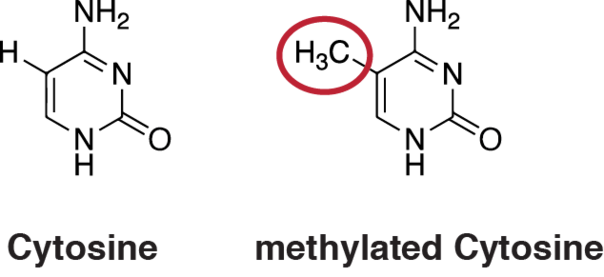
\includegraphics{figs/genome/dna-methylation.png}}
  \caption[6pt]{DNA methylation.}
  \label{fig:g-dna-methylation}
\end{marginfigure}

The lower frequency of \textbf{CG} dinucleotides in the genome is primarily due to the methylation of cytosine, which converts it into 5-methylcytosine. This modification plays a key role in gene silencing and epigenetic regulation. Over evolutionary time, methylated cytosines tend to mutate into thymines (T) through a process called deamination. This mutation leads to a gradual loss of \textbf{CG} dinucleotides from the genome, resulting in fewer \textbf{CpG islands} than would be expected by chance.

This reduction in \textbf{CG} content may have provided evolutionary benefits\marginnote{The discovery of DNA methylation in the 1940s by Rollin Hotchkiss gave rise to the field of epigenetics, which studies changes in gene expression without altering the DNA sequence. These changes, such as the methylation of cytosine in CpG dinucleotides, can silence or reduce gene activity. Importantly, epigenetic modifications can be inherited during cell division and, in some cases, passed from one generation to the next, meaning that environmental factors can influence not only an individual’s gene expression but also potentially affect their offspring.}. Methylation and the resulting mutations likely played a role in genome defense mechanisms, such as \textit{silencing transposable elements} (DNA sequences that can move within the genome) to prevent them from disrupting functional genes. Additionally, selective pressure may have favored a reduced number of CpG dinucleotides outside CpG islands, minimizing unnecessary mutations that could interfere with essential gene regulation processes.

Just one more note about methylation: the mechanism that retains methylation during DNA replication is called maintenance methylation. This process is carried out by an enzyme called DNA methyltransferase 1 (DNMT1). When DNA is replicated, the new strand is synthesized without methylation marks. DNMT1 recognizes hemimethylated DNA (where the parent strand is methylated and the newly synthesized strand is not) and adds methyl groups to the corresponding sites on the new strand. This ensures that the methylation pattern is preserved across cell divisions, thereby maintaining the epigenetic state and regulatory memory of the genome.

Other than CpG, the dinucleotides TpA and CpA are also of interest in genomic studies, each for different reasons:

\begin{itemize}
    \item TpA: This dinucleotide is often underrepresented in genomic sequences, likely due to its association with instability in the DNA double helix. TA pairs form only two hydrogen bonds, making them more prone to mutations and breakage. This dinucleotide also plays a role in certain regulatory regions like promoters and is found in repetitive elements.
    
    \item CpA: CA dinucleotides are frequently found in regions of active gene expression and are often involved in alternative splicing. Methylation of CpA is also emerging as a topic of interest, particularly in non-CpG methylation, which is being linked to developmental and tissue-specific gene regulation.
\end{itemize}

Both of these dinucleotides, along with others, contribute to the broader understanding of DNA sequence evolution, mutability, and regulation of gene expression.

\section{Where to Go from Here}

This chapter offers just a glimpse into the world of genomes and DNA sequences. In the next chapter, we will continue our exploration by focusing on how genes are identified within these sequences and how computational methods can help characterize their structure and function.

\section*{Ideas for Mini Projects}

For simplicity, in all the exercises below, all analyses may be performed using only one strand of the DNA sequence (as provided in the genome file), without considering the reverse complement. Notice that this strand is also referred to as plus strand.

\begin{enumerate}
\item Consider two groups of bacteria: 
\begin{itemize}
\item Group A, free-living and metabolically active: \textit{Mycobacterium tuberculosis} (NCBI accession id \texttt{AL123456.3}), \textit{Pseudomonas aeruginosa} (\texttt{NC\_002516.2}), \textit{Streptomyces coelicolor} (\texttt{NC\_003888.3}),
\item Group B, parasitic or symbiotic: \textit{Mycoplasma genitalium} (\texttt{NC\_000908.2}), \textit{Chlamydia trachomatis} (\texttt{NC\_000117.1}), \textit{Borrelia burgdorferi} (\texttt{NC\_001318.1}), \textit{Helicobacter pylori} (\texttt{NC\_018939.1}).
\end{itemize}
With these two groups, perform the following tasks:
\begin{enumerate}
\item Find out what organisms in Group A have in common, and what organisms in Group B have in common (you may use any chatbot or online resource).
\item Write Python code (using Biopython's Entrez/SeqIO or similar) that loads the genome sequences of these organisms and compares their genome lengths. What differences do you observe?
\item Extend the code to compute the frequency of codons (triplets of nucleotides) for each genome. Do you notice any systematic differences between Group A and Group B?
\item Finally, use biological reasoning (with the help of a chatbot or literature if needed) to explain \textit{why} these differences in genome size and codon usage might exist between the two groups.
\end{enumerate}

\item Fetch the genome sequences of the three shortest non-Y human chromosomes and analyze their nucleotide composition. Compare the frequencies of A/T versus C/G across each chromosome. Do you observe a consistent difference? If so, determine whether this pattern has an evolutionary explanation using AI chatbots or external references.

\item For the genome sequences from the previous exercise (shortest non-Y human chromosomes), compute the frequency of CpG dinucleotides, and their odds ratio (observed vs. expected). Do you observe any interesting pattern? Can you explain it?

\item A plausable hypothesis is that the CpG depletion in the human genome is directly caused by DNA methylation of cytosines in CpG dinucleotides, followed by mutation (C to T), which gradually removes CpG sites over evolutionary time. If this is the case, then this effect should not be present in organisms with no DNA methylation. Examples of such organisms are budding yeast \textit{Saccharomyces cerevisiae} (consider, for instance, chromose I, \texttt{NC\_001216.2}), bacteria \textit{Escherichia coli} (\texttt{NC\_000913}) and nematode \textit{Caenorhabditis elegans} (chromosome I,\texttt{NC\_003370.1}), which has a very low genome methylation rate. Fetch their genomes and analyze if the absence of DNA methylation is reflected in the frequency of CpG dinucleotides. Always compare the observed frequency of CpG dinucleotides with the expected frequency under the multinomial model.

\item Conside the genome of \textit{Escherichia coli} \texttt{NC\_000913}, and compare the observed and expected frequencies of motives \texttt{AAAAA} and \texttt{GGGGG}. Do these motives occur more or less frequently than expected? Was this expected and if so, why? Use AI chatbots or external references to explain the differences.

\item Consider the motif \texttt{GATCC} in the \textit{Escherichia coli} genome. Considering only the plus strand, the observed frequency of this motif is 0.00090, while its expected frequency under the multinomial (independent nucleotide) model is 0.00099 – only slightly higher. In other words, although this motif appears somewhat less often than expected, the difference does not immediately look significant. Investigate this by performing a permutation (randomization) test. Generate, say, 1000 randomized sequences with the same genome length and nucleotide composition, count how often this motif appears in each, and record the propotion of sequences where the count is less than or equal to the observed count. This is the p-value for our test, that is, the probability of observing a count as low as or lower than the observed count in a random sequence.
\end{enumerate}




\chapter{Where Are the Genes?}
\label{ch:genome}

Genes are located on the DNA. :)

But where exactly? At this stage, let's define a gene as a specific region of the genome that contains a sequence of DNA which is transcribed into messenger RNA and subsequently translated into a protein.

By now, you may be familiar with the central dogma of molecular biology, which essentially explains the flow of genetic information: from DNA to RNA to protein. You also know that DNA is made up of two strands, and these strands run in opposite directions, meaning one strand is the reverse complement of the other. Genes can be found on either strand.

DNA and RNA are synthesized in the 5' to 3' direction. This means that during synthesis, a strand is read from 3' to 5' to create a complementary RNA strand. Consider an example fragment of the DNA:

\begin{verbatim}
    5'-TTT GGA TTC CGG-3'
    3'-AAA CCT AAG GCC-5'
\end{verbatim}

The fragment contains two strands: one running from 5' to 3' and the other running from 3' to 5'. Note that RNA can be synthesized from either of these two strands, and the RNA sequence will be the {\em reverse complement} of the DNA sequence. It will be a {\em complement} since the nucleotides pair with their complementary bases (A with U in RNA, T with A, G with C, and C with G), and reverse since the RNA strand is synthesized in the 5' to 3' direction, opposite to the template strand's 3' to 5' direction.

The {\em 5' to 3' strand} is often referred to as the {\em coding strand} (also known as the sense strand) because it has the same sequence as the mRNA, except that thymine is replaced with uracil in RNA. This is the strand that directly reflects the sequence of the resulting protein. The {\em 3' to 5' strand} is referred to as the {\em template strand} (also known as the antisense strand) because it serves as the template for RNA polymerase during transcription. RNA polymerase reads the template strand in the 3' to 5' direction to synthesize mRNA in the 5' to 3' direction.

In databases like {\em NCBI Nucleotide}, sequences are typically provided in the {\em 5' to 3' direction of the coding strand}. This means that the sequences listed usually correspond to the coding (sense) strand, which matches the mRNA sequence that would be produced (with thymine instead of uracil). Therefore, when we retrieve a nucleotide sequence from a database like NCBI, you are usually getting the sequence in the orientation of the coding strand, from the 5' to 3' end.

\section{Reading Frames}

A reading frame is a way of dividing a DNA or RNA sequence into consecutive, non-overlapping sets of three nucleotides, called codons, which correspond to amino acids during protein synthesis. Since each codon is three bases long, there are three possible reading frames for any given sequence, depending on where you start reading. The correct reading frame is crucial, as a shift in the frame can completely change the resulting amino acid sequence and therefore the function of the protein.

Consider again the DNA fragment we have seen before. If we read our sequence from left to right, the bottom strand is our template strand, and the top strand is our coding strand. Depending on which nucleotide we start with, the complementary nucleotides to the template strand are:

\begin{verbatim}
    TTT GGA TTC CGG
    TTG GAT TCG
    TGG ATT CCG
\end{verbatim}

Each sequence
\marginpar{\raggedright
Instead of thymine, the base used in RNA is uracil. We will leave the writing of the sequences as is. The coding tables are most often written in the DNA language.}
above represents the complementary RNA strand for the respective reading frame. Notice also that instead of complementing the template strain, we can read the complement directly from the 5' to 3' strain of the DNA fragment, which is, for that reason, called the coding strain. These three sequences would translate into three different sequences of amino acid sequences:
%
\begin{verbatim}
    Phe - Gly - Phe - Arg
    Leu - Asp - Ser
    Trp - Ile - Pro
\end{verbatim}

\begin{table}[h!]
    \centering
    \small
    \begin{tabular}{|c|c|c|c|c|c|}
    \hline
    \multirow{2}{*}{1st Letter} & \multicolumn{4}{c|}{2nd Letter} & \multirow{2}{*}{3rd Letter} \\ \cline{2-5}
     & T & C & A & G &  \\ \hline
    T & \textbf{TTT} Phe & \textbf{TCT} Ser & \textbf{TAT} Tyr & \textbf{TGT} Cys & T \\
      & \textbf{TTC} Phe & \textbf{TCC} Ser & \textbf{TAC} Tyr & \textbf{TGC} Cys & C \\
      & \textbf{TTA} Leu & \textbf{TCA} Ser & \textbf{TAA} Stop & \textbf{TGA} Stop & A \\
      & \textbf{TTG} Leu & \textbf{TCG} Ser & \textbf{TAG} Stop & \textbf{TGG} Trp & G \\ \hline
    C & \textbf{CTT} Leu & \textbf{CCT} Pro & \textbf{CAT} His & \textbf{CGT} Arg & T \\
      & \textbf{CTC} Leu & \textbf{CCC} Pro & \textbf{CAC} His & \textbf{CGC} Arg & C \\
      & \textbf{CTA} Leu & \textbf{CCA} Pro & \textbf{CAA} Gln & \textbf{CGA} Arg & A \\
      & \textbf{CTG} Leu & \textbf{CCG} Pro & \textbf{CAG} Gln & \textbf{CGG} Arg & G \\ \hline
    A & \textbf{ATT} Ile & \textbf{ACT} Thr & \textbf{AAT} Asn & \textbf{AGT} Ser & T \\
      & \textbf{ATC} Ile & \textbf{ACC} Thr & \textbf{AAC} Asn & \textbf{AGC} Ser & C \\
      & \textbf{ATA} Ile & \textbf{ACA} Thr & \textbf{AAA} Lys & \textbf{AGA} Arg & A \\
      & \textbf{ATG} Met & \textbf{ACG} Thr & \textbf{AAG} Lys & \textbf{AGG} Arg & G \\ \hline
    G & \textbf{GTT} Val & \textbf{GCT} Ala & \textbf{GAT} Asp & \textbf{GGT} Gly & T \\
      & \textbf{GTC} Val & \textbf{GCC} Ala & \textbf{GAC} Asp & \textbf{GGC} Gly & C \\
      & \textbf{GTA} Val & \textbf{GCA} Ala & \textbf{GAA} Glu & \textbf{GGA} Gly & A \\
      & \textbf{GTG} Val & \textbf{GCG} Ala & \textbf{GAG} Glu & \textbf{GGG} Gly & G \\ \hline
    \end{tabular}
    \caption{Genetic code table.}
    \end{table}

We could also use the upper strain of the DNA fragment as the template strain. Let us write it in the 3' to 5' direction, that is, reading it from right to left:

\begin{verbatim}
    3'-GGC CTT AGG TTT-5'
\end{verbatim}

The complementary RNA strand would be:
\begin{verbatim}
    5'-CCG GAA TCC AAA-3'
\end{verbatim}

Using this strain, the three possible reading frames are:

\begin{verbatim}
    CCG GAA TCC AAA
    CGG AAT CCA
    GGA ATC CAA
\end{verbatim}

Which would translate into:

\begin{verbatim}
    Pro - Glu - Ser - Lys
    Arg - Asn - Pro
    Gly - Ile - Gln
\end{verbatim}

To read our DNA fragment,
\marginpar{\raggedright Given a DNA sequence and its reverse complement, we have six reading frames.}
we thus have six possibilities, three for each strain. And we thus get six different amino acid sequences. Let us automate this process using Python code, also to check if our transciptions and translations are correct.

\vspace*{3mm}
\begin{lstlisting}
from Bio.Seq import Seq
from Bio.Data import CodonTable

coding_seq = "TTTGGATTCCGG"

def reading_frame(seq, start):
    """Reading frame of a sequence starting at start position."""
    end = len(seq) - (len(seq[start:]) % 3)
    return seq[start:end]

def translate_reading_frames(seq):
    """Translate the reading frames of a sequence."""
    for i in range(3):
        frame = reading_frame(seq, i)
        rna_seq = Seq(frame).transcribe()
        protein_seq = rna_seq.translate(to_stop=True)
        print(f"Reading Frame {i + 1}:")
        print(f"Nucleotide sequence: {frame}")
        print(f"Amino acid sequence: {protein_seq}")
        print()

translate_reading_frames(coding_seq)
\end{lstlisting}

The code above will output the following:

\vspace*{3mm}
\begin{lstlisting}
Reading Frame 1:
Nucleotide sequence: TTTGGATTCCGG
Amino acid sequence: FGFR

Reading Frame 2:
Nucleotide sequence: TTGGATTCC
Amino acid sequence: LDS

Reading Frame 3:
Nucleotide sequence: TGGATTCCG
Amino acid sequence: WIP
\end{lstlisting}

Whcih is fine, but note that the aminoacids are here represented with single letters. To use the three-letter code, we need to add the following to our code (where appropriate):

\vspace*{3mm}
\begin{lstlisting}
aa_three_letter = {
    'A': 'Ala', 'R': 'Arg', 'N': 'Asn', 'D': 'Asp', 'C': 'Cys',
    'Q': 'Gln', 'E': 'Glu', 'G': 'Gly', 'H': 'His', 'I': 'Ile',
    'L': 'Leu', 'K': 'Lys', 'M': 'Met', 'F': 'Phe', 'P': 'Pro',
    'S': 'Ser', 'T': 'Thr', 'W': 'Trp', 'Y': 'Tyr', 'V': 'Val',
    '*': 'Stop'
}

def translate_to_three_letter(protein_seq):
    return "-".join(aa_three_letter[aa] for aa in protein_seq)

print(f"Final sequence: {translate_to_three_letter(protein_seq)}")
\end{lstlisting}

Let us change the code slightly, and output the translations for all the six reading frames. Notice that, given the coding sequence, we also need to translate all the frames from its reverse complement:

\vspace*{3mm}
\begin{lstlisting}
def translate_reading_frames(seq):
    for i in range(3):
        frame = reading_frame(seq, i)
        rna_seq = Seq(frame).transcribe()
        protein_seq = rna_seq.translate(to_stop=True)
        yield translate_to_three_letter(protein_seq)

reverse_complement = Seq(coding_seq).reverse_complement()
for seq in (coding_seq, reverse_complement):
    print("\n".join(translate_reading_frames(seq)))
\end{lstlisting}

The output now nicely reads:

\vspace*{3mm}
\begin{lstlisting}
Phe-Gly-Phe-Arg
Leu-Asp-Ser
Trp-Ile-Pro
Pro-Glu-Ser-Lys
Arg-Asn-Pro
Gly-Ile-Gln
\end{lstlisting}
%
and matches the translations we have done manually.

\section{Structure of Genes}

A typical gene consists of several key regions that govern its expression
\marginpar{\raggedright 
Gene expression is the process by which information from a gene is used to synthesize a functional product, typically a protein, through transcription and translation.}
and function. The {\em promoter} region contains binding sites for transcription factors and RNA polymerase, which initiate transcription at the {\em transcription start site (TSS)}. The {\em 5' untranslated region (5' UTR)} follows, playing a role in regulating mRNA stability and translation efficiency, though it is not translated into protein. The {\em open reading frame (ORF)} is the main coding region, responsible for producing the protein sequence. After the ORF, the {\em 3' untranslated region (3' UTR)} influences mRNA stability, localization, and translation after transcription. Finally, the {\em polyadenylation signal} signals the addition of a poly-A tail to the mRNA, which enhances its stability and facilitates export from the nucleus.

\begin{figure*}[ht]
    \centering
    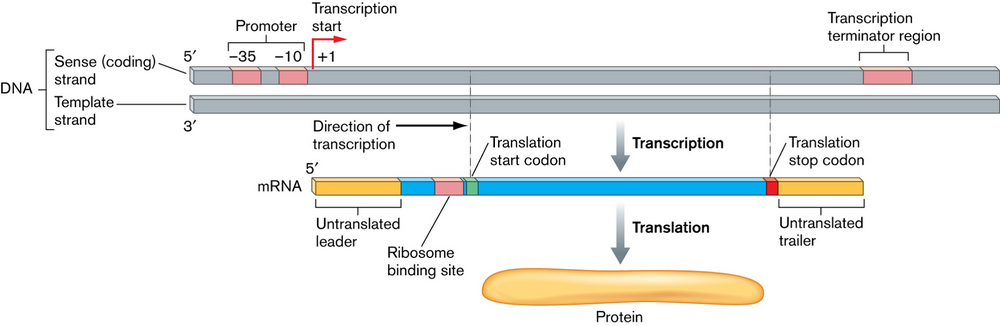
\includegraphics[width=0.99\textwidth]{figs/genes/structure-gene-bacterial.png}
    \caption{A structure of a typical gene.}
    \label{fig:w-gene-structure}
\end{figure*}

Figure~\ref{fig:w-gene-structure} shows a typical gene structure as we have described above. Note that this structure represents a bacterial (prokaryotic) genome, where genes are typically organized without introns. In contrast, in eukaryotic genomes, genes contain introns that are removed during a process called splicing, leaving only exons to form the mature mRNA.

\section{Open Reading Frames}

An {\em open reading frame (ORF)} is a continuous stretch of nucleotides in a DNA sequence that has the potential to be translated into a protein. It begins with a start codon (usually ATG) and extends up to, but does not include, a stop codon (such as TAA, TAG, or TGA), which signals the end of translation. An ORF is different from a {\em reading frame}, which refers to one of the three possible ways in which a nucleotide sequence can be read in sets of three nucleotides (codons). A reading frame becomes an open reading frame only when it includes a start codon, a series of codons that could code for amino acids, and ends with a stop codon, indicating a potential protein-coding sequence. Not all reading frames are open reading frames, as some may not contain both a start and stop codon.

An {\em open reading frame (ORF)} is not necessarily the coding sequence of a gene because the start codon, an {\em ATG}, also encodes the amino acid methionine, which can appear within a gene, not just at the start. This means that an ORF could be part of a larger sequence or occur in non-coding regions where it doesn't correspond to a functional gene. Additionally, regulatory elements and post-transcriptional modifications, like splicing, may result in ORFs that are never translated into functional proteins. Therefore, while ORFs are potential coding sequences, not all ORFs correspond to actual gene-coding regions.


In general, the term ORF can apply to all uninterrupted sequences between a start and stop codon, not necessarily limited to the longest one, as many smaller ORFs may be present within a gene sequence. However, when identifying coding regions, researchers often prioritize the longest ORF as it is more likely to represent the primary protein-coding sequence. For this reason, open reading frame typically refers to the longest possible stretch of DNA (or RNA) between a start codon (often ATG in DNA) and a stop codon (TAA, TAG, or TGA in DNA) that could be translated into a protein. 

\section{Gene Prediction}

{\em Gene prediction} is the process of identifying the location and structure of genes in a genome. This is a crucial step in understanding the genetic information encoded in a genome and is essential for studying gene function, evolution, and disease. Gene prediction can be done using computational methods, which analyze DNA sequences to identify potential genes based on sequence features and patterns.

We will greatly simplify the process of gene prediction here and focus only on finding the longest open reading frames, i.e. the longest stretches between start and any stop codon. Let us start with a Python code that finds all open reading frames in a given DNA sequence.

\vspace*{3mm}
\begin{lstlisting}
from Bio import SeqIO
from Bio.Seq import Seq

def codon_walk(s, frame=0):
    """Walk through a sequence in codons."""
    for ix in range(frame, len(s), 3):
        yield ix, s[ix:ix+3]


def orf_finder(seq, frame, strand=1):
    """Find the longest ORFs in a sequence."""
    orfs = []
    start = None
    n = len(seq)
    for index, codon in codon_walk(seq, frame):
        if not start and codon in START_CODON:
            start = index
        # +3 below for including the stop codon
        elif start and codon in STOP_CODON:
            if strand == 1:
                orfs.append((start, index+3, strand))
            else:
                orfs.append((n-(index+3), n-start, strand))
            start = None
    return orfs

def get_orfs(seq):
    """Get ORFs from a sequence and its reverse complement."""
    orfs = []
    for s, strand in ((seq, 1), (seq.reverse_complement(), -1)):
        for frame in range(3):
            orfs.extend(orf_finder(s, frame, strand))
    return orfs
\end{lstlisting}

The function \texttt{codon\_walk} is a generator that walks through a sequence in codons. The function \texttt{orf\_finder} finds open reading frames in a sequence; it remembers the first occurence of the start codon, and when it hits the stop codon in the current reading frame saves it to the list. The function \texttt{get\_orfs} finds ORFs in a sequence and its reverse complement.

Notice that the stop codon is not a part of ORF, but we included it so that we can easily check which stop codon was encountered, and verify that the code actually works.

Let us test the code first using a really short sequence:

\vspace*{3mm}
\begin{lstlisting}
>>> START_CODON = set(["ATG"])
>>> STOP_CODON = set(["TAA", "TAG", "TGA"])
>>> seq = Seq("AAACTAATGTTTTTTATGTTTTAAAAAAACATA")
>>> orfs = get_orfs(seq)
>>> orfs
[(6, 24, 1), (20, 32, -1)]
>>> for start, end, strand in orfs:
...    print(f"ORF: {start}-{end}, {int((end-start)/3) - 1}"
...    "(strand: {strand})")
...    s = seq[start:end] if strand==1 
...        else seq[start:end].reverse_complement()
...    print(f"{s}")
...    print()
...
ORF: 6-24, 5 (strand: 1)
ATGTTTTTTATGTTTTAA

ORF: 20-32, 3 (strand: -1)
ATGTTTTTTTAA
\end{lstlisting}

This looks ok, but let us test the code on a real genome. We will use the genome of {\em Mycoplasma genitalium}, a bacterium with one of the smallest genomes known for a free-living organism. In {\em M. genitalium}, the TGA codon is unusual because it is typically a stop codon in most organisms, but in this organism, it encodes the amino acid tryptophan (Trp) instead of signaling termination. Therefore, the functional stop codons in M. genitalium are only TAA and TAG.

\vspace*{3mm}
\begin{lstlisting}
>>> seq = SeqIO.read("data/m_genitalium.fasta", "fasta").seq
>>> START_CODON = set(["ATG"])
>>> STOP_CODON = set(["TAA", "TAG"])
>>> orfs = get_orfs(seq)
>>> len(orfs)
10716
\end{lstlisting}

That's a lot of open reading frames! {\em M. genetalium}, in fact, has only about 500 protein-coding genes. So not all of these ORFs are actual genes. And then could also miss some of the 

For a start, we can filter out the ORFs that are too short to be considered protein-coding genes. But how long actully are ORFs that we found? And how long are the actual genes in the genome? It is time to find this out.

\section{ORF Lengths}

First, we start with our ORFs. Remember, we already looked for the longest stretches of DNA between start and stop codons, and were therefore already biased towards longer sequences. But how long are they?

\vspace*{3mm}
\begin{lstlisting}
>>> n = len(orfs)
>>> for i in range(0, 200, 20):
>>>     k = sum(1 for l in lengths if i <= l < i+20)
>>>     print(f"{i:3} .. {i+20:3}: {k:>5,} ({k/n:4.1%})")
  0 ..  20: 7,030 (65.6%)
 20 ..  40: 2,036 (19.0%)
 40 ..  60:   639 (6.0%)
 60 ..  80:   262 (2.4%)
 80 .. 100:   136 (1.3%)
100 .. 120:    92 (0.9%)
120 .. 140:    54 (0.5%)
140 .. 160:    41 (0.4%)
160 .. 180:    42 (0.4%)
180 .. 200:    27 (0.3%)
>>> print(f"ORFs longer than {lmax}: {k:,} ({k/n:4.1%})")
ORFs longer than 200: 354 (3.3%)
\end{lstlisting}

The vast majority of our ORFs are short—--too short, in fact, to be considered protein-coding genes. However, there are also some longer ORFs. Filtering out the shorter ones could be beneficial, but what would be a reasonable length threshold to use? Several approaches can help determine this, and we will examine them one at a time.

\section{Permutation Test}

Start and stop codons are not just randomly placed throughout the genome. At least we hope so. :). Throughout the evolution, the genome been reshaped to contain those codon at the right places so that within them the open reading frames are long enough to be considered genes. Surely, therefore, the distribution of the length of ORFs should be different from the ORFs inferred from some random sequence. We can test this hypothesis using a permutation test.

Let's permute our input sequence, and redo the ORF search.

\vspace*{3mm}
\begin{lstlisting}
import random
seq = list(seq)
random.seed(42)
random.shuffle(seq)
seq = Seq("".join(seq))
orfs = get_orfs(seq)

lengths = [int((end-start)/3-1) for start, end, _ in orfs]
report_length_dist(lengths)
\end{lstlisting}

We packed the code that reports on length distribution within \texttt{report\_length\_dist} (not shown here). Running the code, we get:

\vspace*{3mm}
\begin{lstlisting}
  0 ..  20: 11,133 (68.1%)
 20 ..  40: 3,607 (22.1%)
 40 ..  60: 1,153 (7.1%)
 60 ..  80:   301 (1.8%)
 80 .. 100:   104 (0.6%)
100 .. 120:    35 (0.2%)
120 .. 140:     5 (0.0%)
140 .. 160:     1 (0.0%)
160 .. 180:     0 (0.0%)
180 .. 200:     0 (0.0%)
ORFs longer than 200: 0 (0.0%)
\end{lstlisting}

That's a major difference with the distribution of ORF lengths when these are inferred from the actual, non-permuted sequence. In the permuted sequence, there are no ORFs longer than 200 codons, while in the actual sequence, there are 354 of them. This suggests that the distribution of ORF lengths in the actual sequence is not random and that the ORFs we found are not just random stretches of DNA.

We can use this information to set a threshold for the minimum ORF length. For example, we could set the threshold so that there is only a small chance that an ORF of that length would be found in a permuted sequence. Let us denote this probability as $\alpha$. By setting $\alpha = 0.05$, we indicate that we are willing to accept a 5\% probability of incorrectly identifying a random sequence as an ORF of interest. Thus, we would set the minimum ORF length threshold so that only 5\% of ORFs in a randomly permuted sequence would meet or exceed this length:

\vspace*{3mm}
\begin{lstlisting}
>>> alpha = 0.05
>>> sorted(lengths, reverse=True)[int(len(orfs)*alpha)]
50
\end{lstlisting}

Turns out, in our permutation experiment, we need to set the threshold to 50. Setting $\alpha$ to, say, $0.01$, we would be more stringent and accept only 1\% probability of incorrectly identifying a random sequence as an ORF of interest. The threshold would then be:

\vspace*{3mm}
\begin{lstlisting}
>>> alpha = 0.01
>>> sorted(lengths, reverse=True)[int(len(orfs)*alpha)]
77
\end{lstlisting}

Oh, well, it all depends on our choice of the degree of error we are willing to accept. In one way, we have replaced one problem, one parameter, with another, but at least we now think we understand what is going on and know that our threshold should be set probably in the range from 50 to, say, 100.

\section{Mutlinomial Sequence Model}

Another approach to determining the minimum ORF length threshold is to use a multinomial sequence model. This model assumes that the sequence is generated by a multinomial distribution, with each codon drawn independently from the distribution. We can either estimate the parameters of this distribution from the actual sequence or assume that each codon is equally likely to appear. Let’s proceed with the latter and see where this leads us.

Let us denote the probability of a run of a $k$ or more non-stop codons with $P$, and assert that this probability should be less than $\alpha$, the level of the error we would accept for finding the ORF if the sequence would be random. Assuming all codons are equally likely, and taking into account that there ae (usually) three stop codons, we can write:

$$ P = \binom{61}{64}^k \leq \alpha $$

It is then easy to solve this equation for $k$:

$$ k \geq \frac{\log(\alpha)}{\log(61) - log(64)} $$

With $\alpha = 0.05$, we get $k\approx 63$, and with $\alpha = 0.01$, we get $k\approx 96$. Which matches well with what we have found using the permutation test. Again, given a specific genome, we could be more precise by estimating the actual codon frequencies.

\section{Comparison with Actual Gene Models}

To find an appropriate threshold for the minimum ORF length, we can also compare the ORFs we identified with the actual gene models in the genome. For this purpose, we can consider an organism that has been well-studied and has an annotated genome, meaning the locations of the genes are known. By comparing the ORFs we found, filtered by length, with the actual genes in the genome, we can evaluate how well they match.

We need two main ingredients for this approach: the annotated genome and criteria to assess how closely our ORFs match the actual genes.

Let us start with the first ingredient. The annotated genomes can be accessed in the public databases, such as NCBI, and the following code will do the work, plus it will save the annotations to the local file for later reuse:

\vspace*{3mm}
\begin{lstlisting}
import os
import pickle
from Bio import Entrez

organism_id = {
    "Hs_21q": "BA000005.3",  # H. sapiens chromosome 21q
    "Mt": "AL123456.3",  # Mycobacterium tuberculosis
    "Mg": "NC_000908.2",  # Mycoplasma genitalium
    "Ec": "NC_000913",  # E coli
}

def load_gene_model(organism):
    filename = f"data/{organism}-gb.pickled"
    if os.path.exists(filename):
        # Load the sequence record from the pickle file
        with open(filename, "rb") as f:
            rec = pickle.load(f)
    else:
        # Fetch the sequence from NCBI if not cached locally
        Entrez.email = "your-email-here"
        with Entrez.efetch(
            db="nucleotide",
            rettype="gbwithparts",
            retmode="text",
            id=organism_id[organism]
        ) as handle:
            rec = SeqIO.read(handle, "gb")
        
        # Save the fetched record to a pickle file for future use
        with open(filename, "wb") as f:
            pickle.dump(rec, f)
    return rec
\end{lstlisting}

Let us load the gene model for {\em M. genitalium} and see what kind of features do we have access to:

\vspace*{3mm}
\begin{lstlisting}
>>> model = load_gene_model("Mg")
>>> model.description
'Mycoplasmoides genitalium G37, complete sequence'
>>> len(model.features)
1137
>>> Counter(f.type for f in model.features)
Counter({'gene': 568,
         'CDS': 526,
         'tRNA': 36,
         'rRNA': 3,
         'ncRNA': 2,
         'source': 1,
         'tmRNA': 1})
\end{lstlisting}

Of the features above, there are two that may interest us. The {\em gene} annotation marks the entire region of DNA that defines a gene, including both coding and non-coding regions necessary for its function, such as regulatory elements, exons, and introns. In contrast, the {\em CDS} (Coding Sequence) annotation specifies only the segment that codes for the protein, starting from the start codon and ending at the stop codon, excluding non-coding regions like introns and regulatory sequences. Thus, while the gene encompasses all parts involved in the expression and regulation of a gene product, the CDS is limited to the exact sequence translated into a protein.

For our comparison with the ORFs we found, we therefore need to consider CDS, the coding sequences. There are 526 of them in the {\em M. genitalium} genome. 

Our second ingredient is the criteria for assessing how well our ORFs match the actual genes. To do this, we can use several scoring functions from the field of machine learning. First, we define the following terms:

\begin{itemize}
    \item \textbf{TP} (True Positives): The number of ORFs correctly identified as genes.
    \item \textbf{FP} (False Positives): The number of ORFs incorrectly identified as genes.
    \item \textbf{FN} (False Negatives): The number of actual genes not identified as ORFs.
    \item \#predictions: The total number of predicted ORFs.
    \item \#genes: The total number of actual genes in the annotated genome.
\end{itemize}

Using these definitions, we can calculate:

\begin{itemize}
    \item \textbf{Precision}: The fraction of correctly identified ORFs among all identified ORFs.
    \[
    \text{Precision} = \frac{\text{TP}}{\text{TP} + \text{FP}}
    \]
    
    \item \textbf{Recall}: The fraction of correctly identified ORFs among all actual genes.
    \[
    \text{Recall} = \frac{\text{TP}}{\text{TP} + \text{FN}}
    \]
    
    \item \textbf{F1 Score}: The harmonic mean of precision and recall, balancing the two.
    \[
    \text{F1 Score} = 2 \cdot \frac{\text{Precision} \times \text{Recall}}{\text{Precision} + \text{Recall}}
    \]
\end{itemize}

Here is now our battle plan: we find all the longest ORFs in the genome, then threshold them by length $L$, and compare them with the actual genes in the genome. We will use the F1 score as our main metric to evaluate how well our ORFs match the actual genes. We will then vary the threshold $L$ and see how the F1 score changes. Below, we assume the \texttt{model} and the sequence \texttt{seq} are aready loaded.

\vspace*{3mm}
\begin{lstlisting}
cds = [f for f in model.features if f.type == "CDS"]
orfs = get_orfs(seq)

locs = set((int(c.location.start), int(c.location.end),
            c.location.strand) for c in cds)

print(f"{'L':>3} {'Pred':>4} {'True':>5} {'False':>5} "
      f"{'Prec':>5} {'Rec':>5} {'F1':>5}")
for min_len in range(50, 200, 10):
    sel = [orf for orf in orfs 
           if ((orf[1] - orf[0]) / 3 - 1) > min_len]

    tp = [strand for (s, e, strand) in sel 
          if (s, e, strand) in locs]
    prec = len(tp) / len(sel)
    recall = len(tp) / len(locs)
    f1 = 2 * prec * recall / (prec + recall)
    print(f"{min_len:3d} {len(sel):4d} {len(tp):4d} "
          f"{len(sel) - len(tp):6d} "
          f"{prec:5.3f} {recall:5.3f} {f1:5.3f}")
\end{lstlisting}

Most of the above code is just for the output formatting. The actual calculation of the F1 score is done in the loop. Note also that we store the actual locations of the genes in the set \texttt{locs} for faster lookup. Running the code, we get:

\vspace*{3mm}
\begin{lstlisting}
    L Pred  True False  Prec   Rec    F1
    50 3172 1466   1706 0.462 0.858 0.601
    60 2524 1453   1071 0.576 0.850 0.687
    70 2142 1432    710 0.669 0.838 0.744
    80 1945 1411    534 0.725 0.826 0.772
    90 1798 1383    415 0.769 0.809 0.789
   100 1679 1342    337 0.799 0.785 0.792
   110 1588 1305    283 0.822 0.764 0.792
   120 1522 1274    248 0.837 0.745 0.789
   130 1469 1241    228 0.845 0.726 0.781
   140 1419 1214    205 0.856 0.710 0.776
   150 1371 1174    197 0.856 0.687 0.762
   160 1323 1135    188 0.858 0.664 0.749
   170 1272 1093    179 0.859 0.640 0.733
   180 1228 1057    171 0.861 0.618 0.720
   190 1182 1015    167 0.859 0.594 0.702
\end{lstlisting}

The F1 score is highest for $L=100$, which is consistent with our previous findings. The F1 score is a good metric for evaluating the performance of our ORF prediction, as it balances precision and recall. In this case, the F1 score is highest when the minimum ORF length threshold is set to 100 codons. This threshold gives us a good balance between correctly identifying ORFs and avoiding false positives.

\section{What's Next?}

Admittedly, identifying genes based solely on ORFs and filtering out spurious ones by length is a simplistic approach, though it serves as a good starting point. In reality, gene prediction is a complex process involving additional steps such as identifying promoter regions, splice sites, and regulatory elements. Furthermore, gene prediction often leverages machine learning models that can learn patterns in the data to make more accurate predictions. Here, however, we will stick with our basic approach and move on to the next chapter, where we will explore methods for comparing gene sequences across and within species.
\chapter{Sequence Alignment Methods}
\label{ch:alignment}

Before we can understand how genes evolve and how their functions relate across organisms,  we must first learn how to compare biological sequences in a meaningful way.  The comparison of DNA, RNA, and protein sequences lies at the heart of modern bioinformatics, providing the basis for discovering evolutionary relationships, identifying functional regions, and annotating newly sequenced genomes. Sequence alignment is the systematic arrangement of sequences to reveal their similarities and differences. It serves as the foundation for nearly every computational analysis in molecular biology.

\section{Evolution}

In 1973, evolutionary biologist Theodosius Dobzhansky famously declared that ``nothing in biology makes sense except in the light of evolution.''
\marginnote{Dobzhansky T, {\em Am. Biol. Teacher} {\bf 35}, 125–129 (1973)}.
This statement places evolutionary theory at the center of unifying all aspects of biological science. Evolution provides the framework through which the diversity of life, the complexity of organisms, and the relationships among species can be understood. From molecular genetics to ecology, every biological observation gains coherence when viewed as part of an ongoing process of change driven by variation, inheritance, and natural selection. Without evolution, the facts of biology would remain isolated and inexplicable, with it, they form an integrated picture of life’s history and its continuous adaptation to a changing world.

Evolution 
\marginnote{The concept of evolution predates Darwin, with early ideas of species change proposed by naturalists like Jean-Baptiste Lamarck (1809). However, it was Charles Darwin’s {\em On the Origin of Species} (1859) that unified these ideas with a coherent mechanism—natural selection—supported by extensive evidence. Modern evolutionary biology integrates genetics, paleontology, and molecular biology to describe how life has evolved over billions of years.}
is the process by which populations of organisms change over generations through variation (mutations of their genome), inheritance, and selection. Random mutations introduce genetic diversity, while natural selection favors variants that enhance survival or reproduction. Over time, these gradual changes accumulate, producing the diversity of life observed today. "Over time" here is actually an understatement. Evolution had billions of years in order to shape the life as we know it (Table~\ref{t:history-earth}).

\begin{table}[ht]
\centering
\caption{Key events in the history of Earth and life (Ga $=$ billion years ago; Ma $=$ million years ago; ka $=$ thousand years ago).}
\label{t:history-earth}
\begin{tabular}{ll}
\hline
\textbf{Time (approx.)} & \textbf{Event} \\
\hline
4.54 Ga & Formation of Earth \\
4.0--3.8 Ga & Earliest evidence of life (simple microbial activity) \\
3.5 Ga & Emergence of bacteria and prokaryotic cells \\
2.5--2.0 Ga & Rise of atmospheric oxygen \\
2.1--1.8 Ga & Appearance of eukaryotic cells \\
1.2 Ga & Emergence of multicellular organisms \\
700--600 Ma & First animals (sponges and soft-bodied forms) \\
500--475 Ma & First plants colonize land \\
525--500 Ma & Appearance of vertebrates (jawless fish) \\
400--360 Ma & Transition of vertebrates to land (amphibians) \\
200--150 Ma & Evolution of early mammals alongside dinosaurs \\
7--6 Ma & Emergence of hominins (early human ancestors) \\
300--200 ka & Appearance of modern humans (\textit{Homo sapiens}) \\
\hline
\end{tabular}
\end{table}

Historically, evolution was studied by comparing the morphology, that is, the form and structure of organisms. Evolutionary biologists examined fossils, bones, and visible traits of organisms, and compared these to relate them, finding similarities and differences. With advances in molecular biology, scientists began comparing proteins and DNA sequences, enabling much finer resolution. Computational models, statistical inference, and phylogenetic trees now allow the reconstruction of evolutionary relationships from molecular data.

Gene sequences record the history of evolution at the molecular level. Mutations accumulate over time, leaving detectable patterns of similarity and difference among species. By analyzing these patterns computationally, researchers can infer common ancestry, estimate divergence times, and even predict evolutionary pressures.

\section{Homology}

In evolutionary biology 
\marginnote{Evolutionary biology is the branch of biology that studies the origin, change, and diversification of species over time through mechanisms such as mutation, selection, gene flow, and genetic drift.}
and bioinformatics, homologous genes are genes that share a common ancestral origin. They can be classified into two main types: orthologs and paralogs. Orthologous genes arise from a speciation event, meaning they are found in different species but originated from a single gene in the last common ancestor. These genes typically retain the same function across species, making them key for inferring evolutionary relationships and constructing phylogenetic trees. In contrast, paralogous genes result from a gene duplication event within a genome and may evolve new or specialized functions over time. 

Understanding homology—and distinguishing orthologs from paralogs—is crucial in comparative genomics, because it allows researchers to trace gene evolution, predict gene function across species, and reconstruct the molecular history of life.

A classic example of \textbf{orthologs} is the hemoglobin $\beta$-chain gene in humans and the hemoglobin $\beta$-chain gene in whales (or, equivalently, the myoglobin genes in both species). These genes descended from the same ancestral gene in the last common ancestor of humans and whales and retain similar oxygen-binding functions in their respective species, illustrating how mammals adapted to different environments while conserving core physiological mechanisms. Another striking case involves the \textbf{Hox} genes, which control body-plan development in animals: the same basic set of Hox genes that patterns the body of a fruit fly also guides limb and vertebrae formation in humans.

Paralogs, by contrast, showcase how gene duplication propels innovation. Gene duplication is essentially a genetic accident. It occurs when a segment of DNA is copied twice during replication or recombination. While accidental, such duplications provide extra genetic material that evolution can experiment with — one copy maintains the original function, while the other is free to accumulate mutations and potentially evolve new functions. For example, the human globin genes—$\alpha$-globin and $\beta$-globin—originated from a single ancestral gene but duplicated and diverged to specialize in different parts of the hemoglobin molecule, improving oxygen transport. Similarly, the numerous olfactory receptor genes in humans and other mammals arose from repeated duplications, allowing species to detect a wide range of smells.

These examples illustrate how the study of homologous, orthologous, and paralogous genes reveals the deep evolutionary connections among organisms, and how gene duplication and divergence drive the diversity of life’s molecular machinery. They also motivate us to craft algorithmic means of finding these genes, that is, comparing the genetic sequences within the same and between different organisms. The core techniques for sequence comparison are methods that study sequence alignment.

\section{Sequence Alignments}

To understand relationships between genes or proteins, we need a systematic way to compare their sequences. Sequence alignment is the process of arranging two or more DNA, RNA, or protein sequences to identify regions of similarity that may indicate functional, structural, or evolutionary relationships. Alignments reveal where nucleotides or amino acids correspond between sequences, accounting for possible insertions, deletions, or substitutions that occurred over time. 

Beyond evolutionary studies, sequence alignment underlies many tasks in bioinformatics. These include predicting gene or protein function by similarity to known sequences, identifying coding regions in genomes, assembling overlapping fragments in sequencing projects, constructing phylogenetic trees, and searching for orthologs across species. In essence, alignment transforms raw sequence data into biologically meaningful comparisons, providing the foundation for most computational analyses of molecular biology.

Here is an example. Consider two short DNA sequences $s = \texttt{ATACGTA}$ and $t = \texttt{TATGATA}$. The goal of an alignment $A(s,t)$ is to arrange these sequences so that similar characters are aligned in columns, while gaps (denoted by dashes) represent insertions or deletions that occurred during evolution. A possible (perhaps not a very good) alignment is:

\begin{verbatim}
s:  ATACG-TA
        | ||
t:  TAT-GATA
\end{verbatim}

Here, vertical bars indicate matches between the aligned bases. The alignment reveals that the sequences share several conserved positions, while one gap accommodates an insertion or deletion event. Such visual representations help quantify sequence similarity and form the basis for computational algorithms that compare genes or proteins across species.

Here is another alignment of these two sequences:

\begin{verbatim}
s:  ATACG-TA
     || | ||
t:  -TATGATA
\end{verbatim}

Formally, an alignment of sequences $s$ and $t$ can be represented as
$A(s,t) = (x, y)$, where $x$ and $y$ are the aligned versions of $s$ and $t$,
respectively. Each position in $x$ and $y$ contains either a symbol from the
alphabet (e.g., \texttt{A}, \texttt{C}, \texttt{G}, \texttt{T}) or a gap, and
removing the gaps recovers the original sequences.

Which of the above alignments is better? It depends. :)

\section{Alignment Scoring}

To decide which alignment we like best, we need to define an scoring function over the alignment. Let us denote this function as $M(A(s,t))$. The simplest, and surprisingly the most common way to define the scoring, is to break it down to alignment constituents, that is, defined the function over all aligned positions:
\[
M(A(s,t)) = \sum_{i=1}^{L} \sigma(x_i, y_i),
\]
where $L$ is the alignment length, and $\sigma(x_i, y_i)$ is the
\emph{per-symbol scoring function} that assigns a numerical value depending on
whether the aligned characters at position $i$ are a match, mismatch, or gap.

Typical choices for $\sigma(x_i, y_i)$ include positive scores for matches, negative scores for
mismatches, and penalties for gaps. Say,

\[
\sigma(a,b) =
\begin{cases}
-2, & \text{if } a = \texttt{-} \text{ or } b = \texttt{-}, \\
-1, & \text{if } a \neq b \text{ and } a,b \neq \texttt{-}, \\
+2, & \text{if } a = b.
\end{cases}
\]

The optimal alignment is the one that maximizes $M(A(s,t))$ according to the chosen scoring scheme. With two alignments above, and using this scoring function, the alignment score for the first alignment is $-1$, and for the second alignment $+5$ (see Table~\ref{t:step_by_step_scoring}). Of the two alignments, we would prefer the second one.

\begin{table}[h!]
\centering
\caption{Step-by-step scoring of the alignment $A(s,t)$.}
\label{t:step_by_step_scoring}
\begin{tabular}{ccccc}
\hline
\textbf{Position} & \textbf{$x_i$ (s)} & \textbf{$y_i$ (t)} & \textbf{$\sigma(x_i, y_i)$} & \textbf{Explanation} \\
\hline
1 & A & -- & $-2$ & gap in $t$ \\
2 & T & T  & $+2$ & match \\
3 & A & A  & $+2$ & match \\
4 & C & T  & $-1$ & mismatch \\
5 & G & G  & $+2$ & match \\
6 & -- & A & $-2$ & gap in $s$ \\
7 & T & T  & $+2$ & match \\
8 & A & A  & $+2$ & match \\
\hline
\multicolumn{4}{r}{\textbf{Total:}} & $\displaystyle M(A(s,t)) = +5$ \\
\hline
\end{tabular}
\end{table}

\section{Walks Through Alignment Tables}

We can start with thinking of how to systematically search through different alignments. A search table will do. Consider an example, a sequence $s=\texttt{ATGA}$ and a sequence $t=\texttt{TCA}$, and their alignment 

\begin{verbatim}
s: -  A  T  -  G  A
t: T  -  C  A  -  -
\end{verbatim}

We have to admit that this alignment does not look good in terms of score, but it is still a valid one. It can be obtained through a traversal of the alignment table shown in Table~\ref{t:align-table-1}. In this table, we start in the upper-left corner and must finish in the lower-right corner. The allowed moves are to the cell on the right, which corresponds to taking a symbol from one sequence (say, $t$); to the cell below, which corresponds to taking a symbol from the other sequence (say, $s$); or to the cell diagonally down-right, which corresponds to taking symbols from both sequences and aligning them. Notice that moving right or down introduces an insertion or deletion (indel) into one of the sequences.

\begin{table}[h!]
\centering
\caption{A possible traversal of the alignment table for the sequences $s=\texttt{ATGA}$ and $t=\texttt{TCA}$. The numbers indicate the consecutive steps we take in the table, with (0) indicating a start position and (6) a final position in our alignment walk.}
\label{t:align-table-1}
\begin{tabular}{c|cccc}
\hline
 & \texttt{–} & \texttt{T} & \texttt{C} & \texttt{A} \\
\hline
\texttt{–} & (0) & (1) &  &  \\
\texttt{A} &  & (2) &  &  \\
\texttt{T} &  &  & (3) &  (4) \\
\texttt{G} &  &  &  & (5) \\
\texttt{A} &  &  &  &  (6) \\
\hline
\end{tabular}
\end{table}

We can now score the positions of the alignment, and get $-11$ for an alignment score.

\begin{verbatim}
s: -  A  T  -  G  A
t: T  -  C  A  -  -
  -2 -2 -1 -2 -2 -2
\end{verbatim}

Notice that a different alignment results from a different walk in the alignment table. Consider the following alignment with a walk from a Table~\ref{t:align-table-2}:

\begin{verbatim}
s: -  A  T  G  A  -  -  -
t: T  -  -  -  -  -  C  A
\end{verbatim}

\begin{table}[h!]
\centering
\caption{Another possible traversal of the alignment table for the sequences $s=\texttt{ATGA}$ and $t=\texttt{TCA}$.}
\label{t:align-table-2}
\begin{tabular}{c|cccc}
\hline
 & \texttt{–} & \texttt{T} & \texttt{C} & \texttt{A} \\
\hline
\texttt{–} & (0) & (1) &     &  \\
\texttt{A} &     & (2) &     &  \\
\texttt{T} &     & (3) &     &  \\
\texttt{G} &     & (4) &     &  \\
\texttt{A} &     & (5) & (6) & (7) \\
\hline
\end{tabular}
\end{table}

The scoring of the positions in this alignment is shown below, with the final total score of $-14$, which is even worse than that of our previous alignment:

\begin{verbatim}
s: -  A  T  G  A  -  -  -
t: T  -  -  -  -  -  C  A
  -2 -2 -2 -2 -2 -2 -2 -2
\end{verbatim}

However, notice something important: the two alignments share the same initial part of the walk. Up to position (2), both walks are identical, and therefore the score up to that point (which is $-4$) is the same as well. Once we have computed the score for a particular portion of the walk, there is no need to recompute it if another alignment shares that portion:

\begin{verbatim}
s: -  A | T  -  G  A
t: T  - | C  A  -  -

s: -  A | T  G  A  -  -  -
t: T  - | -  -  -  -  C  A
\end{verbatim}

The total score of the alignment up to the position marked with {\tt |} is $-4$ for both walks. The realization that shared parts of the walk need to be computed only once leads to a very  efficient alignment scoring algorithm—and, ultimately, to an algorithm that can find the  highest-scoring alignment.

\section{A Search for the Best Alignment}

Given two biological sequences, our goal is to find the alignment that achieves the highest possible score according to a chosen scoring scheme. In principle, one could generate \emph{all} possible alignments of the two sequences, compute their scores, and select the best one. However, this exhaustive approach quickly becomes infeasible even for short sequences. For instance, when each sequence has only ten symbols, there are already on the order of $1.9\times 10^5$ possible alignments, and for sequences of length twenty, this number explodes to more than $10^{11}$. A more efficient method is required.

Formally, let $\mathcal{A}(s,t)$ denote the set of all possible alignments between sequences $s$ and $t$. 
For any alignment $A \in \mathcal{A}(s,t)$, let $M(A)$ represent its alignment score. 
The \emph{optimal alignment}, denoted by $A^*(s,t)$, is the alignment that maximizes the scoring function:
\[
A^*(s,t) = \arg\max_{A \in \mathcal{A}(s,t)} M(A),
\qquad
M(A^*) = \max_{A \in \mathcal{A}(s,t)} M(A),
\]
%
so that for all possible alignments $A$,
%
\[
M(A^*) \ge M(A).
\]

A key observation, stemming from our alignment walks above, is that an optimal alignment of two sequences can be built \emph{incrementally}. Suppose we have already computed the best possible alignment for the prefixes of the two sequences up to certain positions. When we extend these prefixes by one additional symbol (or introduce a gap), the best alignment for the longer prefixes can be obtained directly from these previously computed partial results. In other words, the problem exhibits an \emph{optimal substructure}: the optimal solution to the whole problem can be constructed from the optimal solutions to its smaller subproblems.

This insight leads naturally to the \textbf{Needleman–Wunsch algorithm}, 
\marginnote{The Needleman–Wunsch algorithm was introduced by Saul B. Needleman and Christian D. Wunsch in 1970 ({\em Journal of Molecular Biology}) and was the first dynamic programming method for global sequence alignment. It guarantees finding the optimal alignment between two sequences according to a defined scoring scheme and laid the foundation for modern bioinformatics.}
a dynamic programming method that systematically computes the best possible alignment score by filling in a matrix of partial results. We refer to this matrix as the \textbf{dynamic programming table}. Each cell of the table, denoted by $M_{ij}$, represents the best possible alignment score between the prefixes $s_1 s_2 \ldots s_i$ of the first sequence and $t_1 t_2 \ldots t_j$ of the second sequence.

The value of $M_{ij}$ is computed recursively from the neighboring cells, based on whether the last step in the alignment was a match/mismatch, a gap in $s$, or a gap in $t$:

\[
M_{ij} = \max
\begin{cases}
M_{i-1,\,j-1} + \sigma(s_i, t_j), & \text{(align $s_i$ with $t_j$)}\\[6pt]
M_{i-1,\,j} + \sigma(s_i, \texttt{-}), & \text{(gap in $t$)}\\[6pt]
M_{i,\,j-1} + \sigma(\texttt{-}, t_j), & \text{(gap in $s$)}.
\end{cases}
\]

The first row and column of the matrix are initialized with cumulative gap penalties, and the final cell $M_{mn}$ (where $m$ and $n$ are the lengths of the sequences) gives the score of the optimal global alignment. It also helps us if we remember which of the three moves is the one we took to get the maximum value at each particular cell. 


\begin{table}[h!]
\centering
\caption{Dynamic programming table with scores $M_{ij}$ for $s=\texttt{ATGA}$ and $t=\texttt{TCA}$.}
\label{t:dpt}
\begin{tabular}{c|cccc}
\hline
 & \texttt{–} & \texttt{T} & \texttt{C} & \texttt{A} \\
\hline
\texttt{–} & \textbf{0}  & -2 & -4 & -6 \\
\texttt{A} & \textbf{-2} & -1 & -3 & -1 \\
\texttt{T} & -4 & \textbf{0} & -2 & -2 \\
\texttt{G} & -6 & -2 & \textbf{-1} & -3 \\
\texttt{A} & -8 & -4 & -3 & \textbf{-1} \\
\hline
\end{tabular}
\end{table}

Consider the dynamic programming table for the alignment of our two sequences (Table~\ref{t:dpt}). The numbers marked in bold indicate a path we take for optimal alignment. Based on the optimal walk through this table, we find that the optimal alignment is
\begin{verbatim}
s: A  T  G  A
      |  |  |
t: -  T  C  A
\end{verbatim}
and its score is $+1$.

It is important to note that, in some cases, more than one move may yield the same optimal value for a given cell in the dynamic programming table. Such \emph{ties} indicate that multiple paths can lead to the same overall alignment score. Consequently, there may exist several distinct alignments that all achieve the optimal score. In practice, one of these paths can be chosen arbitrarily when tracing back through the table, since all represent equally optimal solutions under the given scoring scheme.

\section{A Note on Dynamic Programming}

Dynamic programming, a term coined by Richard Bellman in the 1950s,
\marginnote{\raggedright Bellman, R. (1952). On the Theory of Dynamic Programming. {\em Proc. of the National Academy of Sciences of the USA}, 38(8), 716–719.} is named to describe a method of solving complex problems by breaking them down into simpler subproblems. Bellman chose the term "dynamic programming" for strategic reasons. At the time, he was working with the U.S. government, where the word "programming" was a popular term and had positive associations, particularly in operations research and planning. By adding "dynamic," he aimed to emphasize the method's focus on time-evolving processes, as the problems it addressed often involved sequences of decisions over time.

In dynamic programming, 
\marginnote{Needleman and Wunsch were aware of Richard Bellman’s work on dynamic programming and based their method directly on his principle of optimality. They were the first to apply dynamic programming to biological sequence alignment, which made their 1970 paper so influential.}
solutions to subproblems are stored (or "memorized") to avoid redundant calculations, which makes it particularly efficient for problems with overlapping subproblems, like shortest path, sequence alignment, and optimization problems. The approach dynamically combines solutions to smaller subproblems to build up the solution to the original, larger problem, leading to a highly structured and systematic way of tackling complex problems.

\section{Local Alignment}

While the Needleman--Wunsch algorithm 
\marginnote{Smith and Waterman built directly on the Needleman–Wunsch algorithm. In their 1981 paper ({\em J. Mol. Biol.}), they added a simple zero term to the recurrence, converting global alignment into local alignment and enabling detection of high-scoring subsequence matches.}
searches for the best \emph{global} alignment between two complete sequences, many biological problems require identifying regions of local similarity instead. For example, two proteins may share only one conserved domain or motif, while the rest of their sequences differ substantially. The goal of \textbf{local alignment} is therefore to find the pair of subsequences that produce the highest alignment score, rather than aligning the sequences end to end. This approach was formalized by \textbf{Smith and Waterman} in 1981, who modified the dynamic programming formulation to reset negative scores to zero, ensuring that only high-scoring local regions are extended. Local alignment is particularly useful for database searches and for detecting conserved functional regions within otherwise unrelated sequences.

The recurrence relation for the local alignment score is defined as:

\[
M_{ij} = \max
\begin{cases}
0, & \text{(start a new alignment)}\\[6pt]
M_{i-1,\,j-1} + \sigma(s_i, t_j), & \text{(match or mismatch)}\\[6pt]
M_{i-1,\,j} + \sigma(s_i, \texttt{-}), & \text{(gap in $t$)}\\[6pt]
M_{i,\,j-1} + \sigma(\texttt{-}, t_j), & \text{(gap in $s$)}.
\end{cases}
\]

By including the zero term, the algorithm discards regions with negative cumulative scores
and effectively identifies the highest-scoring subsequence pair. The maximum value in the
matrix corresponds to the optimal local alignment score, and a traceback starting from that
cell reveals the aligned region.



Here is an example. Consider two sequences, $s =$ \texttt{ACCTGAA} and $t =$ \texttt{CGTGACG}, and the scoring function:
\[
\sigma(a,b) =
\begin{cases}
+2, & \text{if } a = b,\\[4pt]
-1, & \text{if } a \neq b,\\[4pt]
-2, & \text{if } a = \texttt{-} \text{ or } b = \texttt{-}.
\end{cases}
\]

Applying the Smith--Waterman algorithm gives the dynamic programming table shown in Table~\ref{t:smith-waterman}. 
The maximum value in the table (\textbf{8}) corresponds to the best local alignment between the two sequences.

\begin{table}[h!]
\centering
\caption{Dynamic programming table for local alignment of $s=\texttt{ACCTGAA}$ and $t=\texttt{CGTGACG}$. 
The bold numbers indicate the cells on an optimal local-alignment path.}
\label{t:smith-waterman}
\begin{tabular}{c|cccccccc}
\hline
 & \texttt{–} & \texttt{C} & \texttt{G} & \texttt{T} & \texttt{G} & \texttt{A} & \texttt{C} & \texttt{G} \\
\hline
\texttt{–} & 0 & 0 & 0 & 0 & 0 & 0 & 0 & 0 \\
\texttt{A} & 0 & 0 & 0 & 0 & 0 & 2 & 0 & 0 \\
\texttt{C} & 0 & \textbf{2} & 0 & 0 & 0 & 0 & 4 & 2 \\
\texttt{C} & 0 & 2 & \textbf{1} & 0 & 0 & 0 & 2 & 3 \\
\texttt{T} & 0 & 0 & 1 & \textbf{3} & 1 & 0 & 0 & 1 \\
\texttt{G} & 0 & 0 & 2 & 1 & \textbf{5} & 3 & 1 & 2 \\
\texttt{A} & 0 & 0 & 0 & 1 & 3 & \textbf{7} & 5 & 3 \\
\texttt{A} & 0 & 0 & 0 & 0 & 1 & 5 & 6 & 4 \\
\hline
\end{tabular}
\end{table}

The highest-scoring cell (in bold) has a value of $7$, marking the end of the best local alignment. 
Tracing back from that cell reveals the following aligned subsequences:

\begin{verbatim}
s: A C C T G A A
     |   | | |
t:   C G T G A C G
\end{verbatim}

Thus, the Smith--Waterman algorithm identifies the local region \texttt{CCTGA} in $s$ and \texttt{CGTGA} in $t$ as the best-matching subsequences, with an optimal local alignment score of $7$.


\section{An Example: Longest Common Subsequence}

Let us now diverge a bit, and instead of alignments use dynamic programming for a similar problem of finding the longest common subsequence. The \textbf{longest common subsequence (LCS)} of two sequences is the longest sequence that appears in both of them in the same order, but not necessarily contiguously. For example, for $s=\texttt{ACDBE}$ and $t=\texttt{ABCDE}$, the longest common subsequence is $\texttt{ACDE}$, which has length four. The LCS problem captures the idea of sequence similarity without considering insertions, deletions, or substitutions explicitly, and serves as a simplified model for understanding alignment algorithms.

We first need to define the scoring mechanism for traversal of the dynamic programming table. We do not gain in the length of the longest common subsequence if we take only a symbol from one of the sequences, but we gain a length of $1$ if we take symbols from both sequences and they are equal. This can be expressed using a simple scoring function
\[
\sigma(a,b) =
\begin{cases}
1, & \text{if } a = b,\\[4pt]
0, & \text{if } a \neq b.
\end{cases}
\]
The recurrence relation for computing the entries of the dynamic programming table is then
\[
M_{ij} = \max
\begin{cases}
M_{i-1,\,j-1} + \sigma(s_i, t_j), & \text{(take both symbols)}\\[6pt]
M_{i-1,\,j}, & \text{(skip a symbol from $s$)}\\[6pt]
M_{i,\,j-1}, & \text{(skip a symbol from $t$)}.
\end{cases}
\]

Now to the code. We first define the scoring function:

\vspace*{3mm}
\begin{lstlisting}
def score(a, b):
    return 1 if a == b else 0
\end{lstlisting}

This was easy. Now, the main algorithm, the construction of the dynamic programming table. We use a trick: besides computing the scores we will also remember the neighboring cells (up and to the left) from which these scores originated. This will allow us to trace back for the solution of the problem:

\vspace*{3mm}
\begin{lstlisting}
def longest_common_subsequence(s, t):
    M = defaultdict(int)
    P = {}
    for i, si in enumerate(s):
        for j, tj in enumerate(t):
            M[i, j], P[i, j] = max(
                (M[i-1, j], (i-1, j)),
                (M[i, j-1], (i, j-1)),
                (M[i-1, j-1] + score(si, tj), (i-1, j-1))
            )
    return M, P
\end{lstlisting}

After filling in the dynamic programming table $M$, we must recover the actual longest common subsequence by retracing the path of decisions that led to the optimal score. We do this by following the pointers stored in $P$, which indicate which previous cell contributed to the current maximum:

\vspace*{3mm}
\begin{lstlisting}
def trace_back(s, t, M, P):
    i = len(s)-1
    j = len(t)-1
    result = ""
    while M[i, j] != 0:
        if P[i, j] == (i - 1, j - 1):
            result = s[i] + result
        i, j = P[i, j]
    return result
\end{lstlisting}

Finally, we can run the algorithm on two example sequences and display the result:

\vspace*{3mm}
\begin{lstlisting}
s = "AACCTTGG"
t = "ACACTGTGA"
table, previous = longest_common_subsequence(s, t)
substring = trace_back(s, t, table, previous)
print(f"Longest common subsequence: {substring}")
print(f"Length: {table[len(s) - 1, len(t) - 1]}")

\end{lstlisting}

The program outputs:

\vspace*{3mm}
\begin{lstlisting}
Longest common subsequence: AACTTG
Length: 6
\end{lstlisting}

It works! This example demonstrates how dynamic programming can efficiently recover not only the score but also the actual subsequence representing the shared structure between two sequences. The reader can now extend the code to output the actual dynamic programming table, show its entries and highlight the optimal path.

\section{Alignment with Affine Gap Penalties}

So far, we have assumed that each gap in an alignment incurs a linear penalty proportional to its length. 
However, in biological sequences, it is often more realistic to distinguish between the cost of \emph{opening} a gap 
and the cost of \emph{extending} it. Introducing a new gap typically reflects a separate mutational event and 
should therefore be penalized more heavily than simply extending an existing one. 

To capture this, we define an \textbf{affine gap penalty function}:
\[
\gamma(g) = -(\rho + \varepsilon \times x),
\]
where $\rho$ is the cost of \emph{opening} a gap, $\varepsilon$ is the cost of \emph{extending} a gap by one symbol, 
and $x$ is the length of the gap. For example, if $\rho = 5$ and $\varepsilon = 1$, then a gap of length three 
would have a penalty of $-(5 + 3\times1) = -8$. This scheme penalizes multiple short gaps more severely than 
a single long one, which better reflects biological reality.

A simple dynamic programming table, as used in the Needleman–Wunsch algorithm, is insufficient for affine gap penalties. 
That approach assumes that each cell depends only on the immediately adjacent cells (diagonal, above, and left). 
With affine gaps, however, we must distinguish between whether we are \emph{continuing} a gap or 
\emph{starting} a new one. This requires keeping track of the direction from which we arrived at each cell.

To handle this, we maintain three separate dynamic programming matrices:
\[
\begin{cases}
M_{ij}^\downarrow & \text{(gap in $t$ — moving down)},\\[4pt]
M_{ij} & \text{(match or mismatch — moving diagonally)},\\[4pt]
M_{ij}^\rightarrow & \text{(gap in $s$ — moving right)}.
\end{cases}
\]

Each of these matrices represents the best possible score of an alignment ending at position $(i,j)$ 
under the given condition. Their recurrences are defined as follows:

\[
M_{ij}^\downarrow = \max
\begin{cases}
M_{i-1,\,j}^\downarrow - \varepsilon, & \text{(extend a gap in $t$)}\\[4pt]
M_{i-1,\,j} - \rho, & \text{(open a new gap in $t$)}
\end{cases}
\]

\[
M_{ij}^\rightarrow = \max
\begin{cases}
M_{i,\,j-1}^\rightarrow - \varepsilon, & \text{(extend a gap in $s$)}\\[4pt]
M_{i,\,j-1} - \rho, & \text{(open a new gap in $s$)}
\end{cases}
\]

\[
M_{ij} = \max
\begin{cases}
M_{i-1,\,j-1} + \sigma(s_i, t_j), & \text{(match or mismatch)}\\[4pt]
M_{ij}^\downarrow, & \text{(from a gap in $t$)}\\[4pt]
M_{ij}^\rightarrow, & \text{(from a gap in $s$)}.
\end{cases}
\]

Together, these three matrices correctly account for affine gap penalties, 
allowing the algorithm to distinguish between opening and extending gaps 
while still guaranteeing an optimal alignment through dynamic programming.

The traversal for finding the best alignment score now involves moving \emph{across all three matrices} rather than within a single one. At each position $(i,j)$, the algorithm considers transitions not only from neighboring cells within the same matrix but also from corresponding cells in the other two matrices. The optimal path, therefore, may switch between $M_{ij}$, $M_{ij}^\downarrow$, and $M_{ij}^\rightarrow$, depending on whether the alignment continues a match, opens a new gap, or extends an existing one.  The traceback procedure follows this combined path across the three matrices, starting from the cell with the highest overall score and reconstructing the optimal alignment by identifying, step by step, which operation (match, gap opening, or gap extension) was taken. This traversal is illustrated schematically in Figure~\ref{f:affine-gap-traversal}.

\begin{figure}[ht]
    \centering
    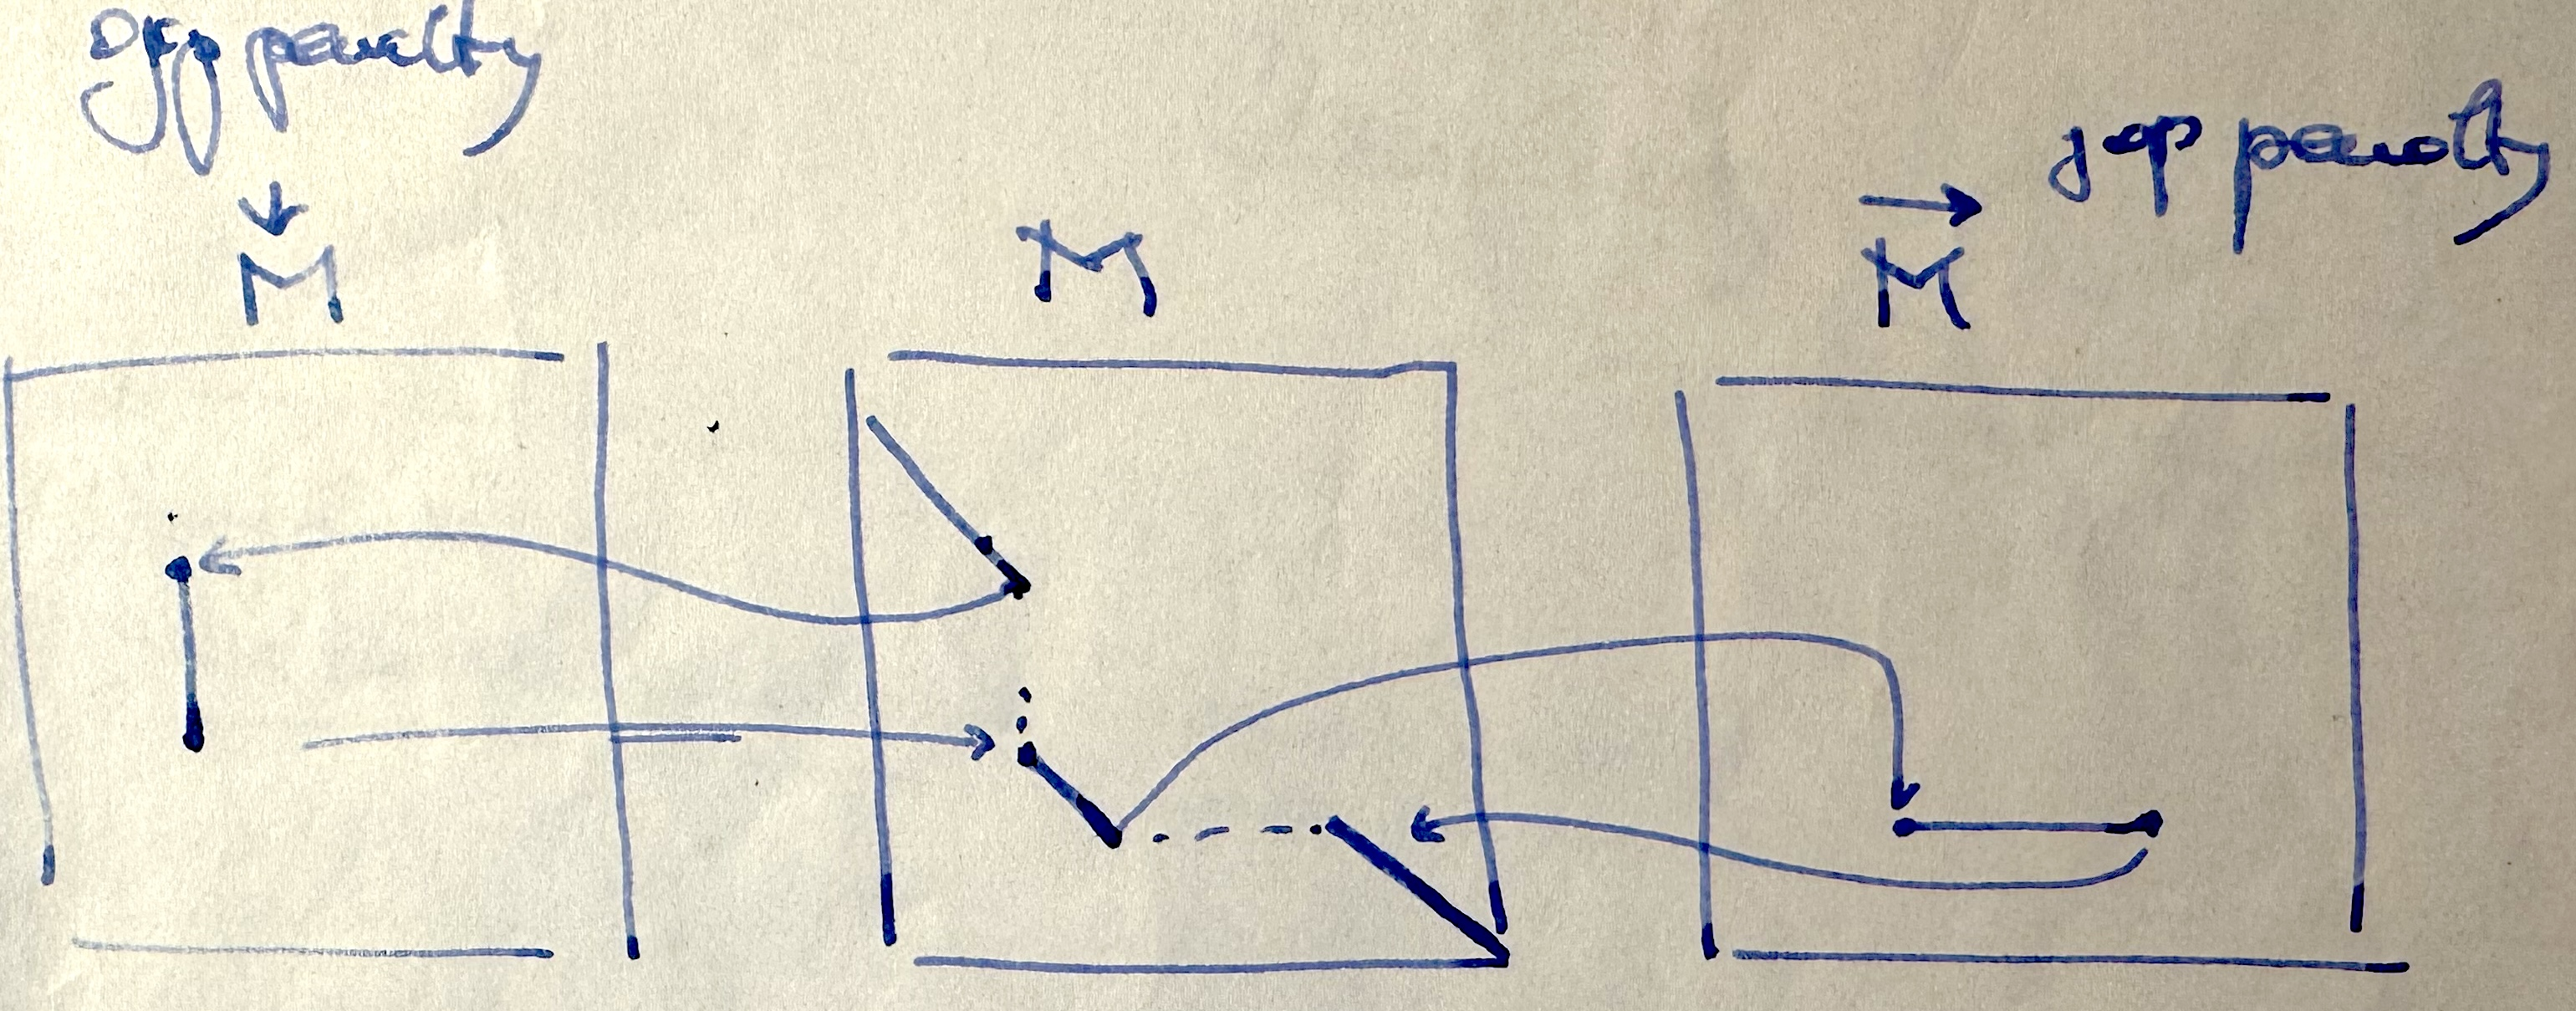
\includegraphics[width=0.99\textwidth]{figs/alignment/affine.jpg}
    \caption{An example of traversal of the three dynamic programming tables for the alignment with affine gap penalties.}
    \label{f:affine-gap-traversal}
\end{figure}

\section{Multiple Sequence Alignment}

Pairwise alignment methods, such as the Needleman–Wunsch and Smith–Waterman algorithms, form the basis of comparing two sequences optimally. However, many biological analyses require comparing whole families of sequences simultaneously. Extending these ideas to three or more sequences leads to the problem of multiple sequence alignment, which generalizes pairwise alignment but introduces new computational challenges. Such comparisons may consider different versions of a gene across species or members of a protein family within the same organism. To reveal regions that have remained similar over time and to understand how the sequences relate evolutionarily, we align all of them together in what is called a multiple sequence alignment. 

A multiple sequence alignment arranges three or more sequences in a table so that symbols with a shared evolutionary origin appear in the same column. For example:
%
\begin{verbatim}
s1: A T - G C A
s2: A T G G - A
s3: A T T G C A
\end{verbatim}
%
This alignment highlights conserved positions (“A–T–G–A”) and regions that have changed through mutations, insertions, or deletions. 

The Needleman--Wunsch algorithm can, in principle, be extended to align more than two sequences. Instead of filling a two-dimensional dynamic programming table, we would construct a table with one dimension for each sequence, where each cell represents the best alignment score for the corresponding prefixes of all sequences. For three sequences, this becomes a three-dimensional cube; for four, a four-dimensional hypercube, and so on. Each additional sequence therefore adds another dimension to the computation. The number of possible paths through this multidimensional table grows exponentially, requiring both time and memory on the order of $O(n^k)$, where $n$ is the sequence length and $k$ is the number of sequences. While this exact dynamic programming approach guarantees an optimal multiple sequence alignment, it quickly becomes impractical. As a result, nearly all practical methods rely on heuristics or approximations that trade exact optimality for tractable computation.

Because exact multiple sequence alignment by dynamic programming is computationally infeasible for more than a few short sequences, practical methods rely on heuristics that approximate the optimal result. One of the most common strategies is progressive alignment. Instead of aligning all sequences at once, the algorithm builds the alignment step by step. First, all pairs of sequences are aligned to estimate their similarities, which are then used to construct a guide tree 
\marginnote{The construction of the guide tree relies on pairwise sequence similarities and forms the basis for clustering algorithms such as \textit{neighbor joining}, which can infer phylogenetic relationships among sequences. We will explore these methods in a later chapter.}
representing their approximate relationships. The two most similar sequences are aligned first, and the resulting alignment is treated as a single entity called a profile.  

A profile summarizes each column of the current alignment by recording how often each nucleotide or amino acid appears there. When a new sequence is added, it is aligned against this profile rather than against individual sequences, choosing the placement that best matches the column frequencies. The process continues until all sequences have been incorporated.  

For example, given three DNA sequences  
\[
\texttt{s}_1 = \texttt{ATGA}, \quad 
\texttt{s}_2 = \texttt{ATGCA}, \quad 
\texttt{s}_3 = \texttt{ATGGA},
\]
the algorithm might first align $\texttt{s}_1$ and $\texttt{s}_2$:
\begin{verbatim}
s1: A T G - A
s2: A T G C A
\end{verbatim}
The resulting profile represents each column as a distribution of residues (for instance, the fourth column has 50\% gaps and 50\% C). The third sequence, $\texttt{s}_3$, is then aligned against this profile to produce the final multiple alignment.

The quality of such an alignment is often measured by the \textbf{sum-of-pairs score}, which adds the scores of all pairwise comparisons implied by the alignment. Columns with matching or chemically similar residues contribute positively, while mismatches and gaps reduce the total.  

An alternative, information-based measure uses \textbf{entropy} to quantify conservation within each column:
\[
H = -\sum_{i=1}^{k} p_i \log_2 p_i,
\]
where $p_i$ is the frequency of residue $i$ and $k$ is the alphabet size. A completely conserved column, where all sequences have the same residue, has $H = 0$; a highly variable one has higher entropy. For example, if 8 out of 10 residues in a column are A and 2 are G, then $H \approx 0.72$.  

Low-entropy columns signal conserved, biologically important regions, while high-entropy columns mark variable positions. Together, these scoring schemes provide complementary ways to evaluate the quality of a multiple sequence alignment, balancing sequence similarity with biological relevance.

Multiple sequence alignments provide the foundation for many downstream analyses in bioinformatics. They are used to identify conserved motifs that indicate important structural or functional sites, to build phylogenetic trees that reconstruct evolutionary relationships, and to generate profiles or hidden Markov models for sequence classification. High-quality alignments are thus critical inputs for comparative genomics, structural prediction, and protein family analysis.

\section{A Note on Scoring Functions for Nucleotide Alignment}

When aligning nucleotide sequences, the scoring function determines the numerical reward or penalty assigned to each possible pairing of nucleotides or gaps. The choice of scoring system has a strong influence on the resulting alignment, especially when gaps are present or when substitution biases exist in the data.

The scoring function we have used above (match = +2, mismatch = -1, gap = -2) is a simple symmetric scheme that treats all nucleotide substitutions equally and applies a uniform penalty for gaps. It assumes that all substitutions and all gaps are equally costly.  While it may is sufficient for illustrating the mechanics of global or local alignment algorithms such as Needleman–Wunsch or Smith–Waterman, in biological data, however, substitutions between nucleotides are not all equally likely.  For instance, in DNA or RNA, the four bases (A, C, G, and T or U) exhibit a strong transition/transversion bias:

\begin{itemize}
    \item Transitions (A$\leftrightarrow$G and C$\leftrightarrow$T) occur more frequently,
    \item Transversions (A$\leftrightarrow$C, A$\leftrightarrow$T, G$\leftrightarrow$C, G$\leftrightarrow$T) occur less frequently.
\end{itemize}

To reflect this bias, one can design a substitution matrix in which transitions are penalized less heavily than transversions. In scoring Table~\ref{tab:nt_substitution_matrix}, transitions (A$\leftrightarrow$G, C$\leftrightarrow$T) receive a penalty of $-0.5$, while transversions are penalized by $-1.5$.

\begin{table}[htbp]
\caption{Example of a nucleotide substitution matrix reflecting transition bias.}
\label{tab:nt_substitution_matrix}
\centering
\begin{tabular}{c|rrrr}
  & A & C & G & T \\
  \hline
  A & +1 & -1.5 & -0.5 & -1.5 \\
  C & -1.5 & +1 & -1.5 & -0.5 \\
  G & -0.5 & -1.5 & +1 & -1.5 \\
  T & -1.5 & -0.5 & -1.5 & +1 \\
\end{tabular}
\end{table}

More sophisticated scoring functions can be derived empirically.
\marginnote{An alternative is to use explicit substitution models such as Kimura models that describe the evolutionary processes with parameters like the transition/transversion ratio and base frequencies. More on such models in later chapters.}
For instance, from a large collection of trusted alignments, say, from a library of homologous sequences, one can estimate the joint probability $P(a,b)$ of observing nucleotides $a$ and $b$ aligned to each other.  The resulting log-odds score is
\begin{equation}
S(a,b) = \lambda \log \frac{P(a,b)}{P(a)P(b)},
\end{equation}
where $P(a)$ and $P(b)$ are background frequencies and $\lambda$ is a scaling constant.

This is analogous to how PAM or BLOSUM matrices (see below) are derived for proteins, though in practice it is less common for DNA because of its smaller alphabet.

There are, however, typical parameter choices for scoring function, depending on the application. Table~\ref{tab:typical_params} summarizes commonly used scoring systems for nucleotide sequence alignment.

\begin{table}[h]
\caption{Common scoring schemes for nucleotide alignment.}
\label{tab:typical_params}
\begin{tabular}{lccc}
\toprule
Purpose & Match & Mismatch & Gap penalty \\
\midrule
Didactic / simple & +2 & --1 & --2 per gap \\
Stringent (identity) & +1 & --3 & --2 per gap  \\
Transition-aware & +5 & --4 transition & --16 open \\
& & --10 transversion & --4 extend \\
\bottomrule
\end{tabular}
\end{table}

\section{Aligning Protein Sequences}

All the examples above included alignments of nucleotide (DNA or RNA) sequences. This is often useful for studying genes and regulatory regions, whereas aligning of protein sequences can provide a deeper understanding of biological function and evolution. 

Protein sequences evolve more slowly at the amino acid level than their corresponding nucleotide sequences since multiple codons can encode the same amino acid. As a result, proteins often retain detectable similarity long after the underlying DNA sequences have diverged beyond recognition. Aligning protein sequences therefore allows us to identify conserved structural and functional regions—such as catalytic sites, binding motifs, or folding domains—that may be invisible in nucleotide-level comparisons.

Protein alignments are especially valuable when comparing genes from different species (homology detection), inferring evolutionary relationships, or annotating new genes based on known protein families. They are also used in structural biology and drug discovery to predict the function of uncharacterized proteins or to design mutations that alter activity or stability. Aligning protein sequences, however, introduces additional complexity: there are twenty amino acids rather than four nucleotides, and not all mismatches are equally likely or equally significant. To align proteins effectively, we must define an appropriate scoring mechanism that reflects biochemical and evolutionary relationships among amino acids.

\section{Protein Substitution Matrices}

Protein substitution matrices are essential in bioinformatics, particularly for scoring alignments between protein sequences by assessing the likelihood of amino acid substitutions that may have occurred over time. Among the most widely used of these is the BLOSUM (BLOcks SUbstitution Matrix),
\marginnote{The BLOSUM matrices were introduced by Steven and Jorja Henikoff in 1992 in their paper ``Amino acid substitution matrices from protein blocks,'' published in \emph{Proceedings of the National Academy of Sciences of the USA} (PNAS).}
which is derived from highly conserved regions, or “blocks,” of protein families. By analyzing these regions that remain largely unchanged across evolution, BLOSUM matrices help detect similarity between protein sequences and reveal functional or structural relationships.

The BLOSUM matrices were derived from data in the BLOCKS database, which contained about 500 conserved regions, or "blocks," from approximately 200 protein families.
\marginnote{A protein family is a group of proteins that share a common evolutionary origin, often re\-flected in similar structures, functions, or sequence motifs.} 
Each block represented a stable, functionally important region within a protein family that has remained largely unchanged over evolutionary time. By focusing on these conserved regions with minimal variation, researchers could analyze meaningful substitutions that likely reflect evolutionary relationships. This made the BLOCKS database an ideal resource for deriving substitution scores that capture genuine evolutionary patterns.

To create BLOSUM matrices,
\marginnote{In BLOSUM matrix construction, similarity is measured as the percentage of identical amino acids between sequences within an aligned, gap-free block, where all sequences are of the same length.}
sequences within each block were grouped, or "clustered," according to a specific similarity threshold. Clustering in this context means that sequences within a block that share more than the specified percentage of similarity (e.g., 62\% for BLOSUM62) are grouped together as a single "cluster." Substitutions are then only counted between different clusters rather than within a cluster, reducing the influence of closely related sequences and emphasizing broader evolutionary changes. By capturing substitutions across clusters, BLOSUM matrices can better detect relationships in distantly related proteins.

\begin{table}[tbp]
\caption{BLOSUM62 matrix.}
\label{tab:blosum62}
\footnotesize
\[
\begin{array}{c|rrrrrrrrrrrrrrrrrrrr}
   & A  & R  & N  & D  & C  & Q  & E  & G  & H  & I  & L  & K  & M  & F  & P  & S  & T  & W  & Y  & V \\
\hline
A  &  4 & -1 & -2 & -2 &  0 & -1 & -1 &  0 & -2 & -1 & -1 & -1 & -1 & -2 & -1 &  1 &  0 & -3 & -2 &  0 \\
R  & -1 &  5 &  0 & -2 & -3 &  1 &  0 & -2 &  0 & -3 & -2 &  2 & -1 & -3 & -2 & -1 & -1 & -3 & -2 & -3 \\
N  & -2 &  0 &  6 &  1 & -3 &  0 &  0 &  0 &  1 & -3 & -3 &  0 & -2 & -3 & -2 &  1 &  0 & -4 & -2 & -3 \\
D  & -2 & -2 &  1 &  6 & -3 &  0 &  2 & -1 & -1 & -3 & -4 & -1 & -3 & -3 & -1 &  0 & -1 & -4 & -3 & -3 \\
C  &  0 & -3 & -3 & -3 &  9 & -3 & -4 & -3 & -3 & -1 & -1 & -3 & -1 & -2 & -3 & -1 & -1 & -2 & -2 & -1 \\
Q  & -1 &  1 &  0 &  0 & -3 &  5 &  2 & -2 &  0 & -3 & -2 &  1 &  0 & -3 & -1 &  0 & -1 & -2 & -1 & -2 \\
E  & -1 &  0 &  0 &  2 & -4 &  2 &  5 & -2 &  0 & -3 & -3 &  1 & -2 & -3 & -1 &  0 & -1 & -3 & -2 & -2 \\
G  &  0 & -2 &  0 & -1 & -3 & -2 & -2 &  6 & -2 & -4 & -4 & -2 & -3 & -3 & -2 &  0 & -2 & -2 & -3 & -3 \\
H  & -2 &  0 &  1 & -1 & -3 &  0 &  0 & -2 &  8 & -3 & -3 & -1 & -2 & -1 & -2 & -1 & -2 & -2 &  2 & -3 \\
I  & -1 & -3 & -3 & -3 & -1 & -3 & -3 & -4 & -3 &  4 &  2 & -3 &  1 &  0 & -3 & -2 & -1 & -3 & -1 &  3 \\
L  & -1 & -2 & -3 & -4 & -1 & -2 & -3 & -4 & -3 &  2 &  4 & -2 &  2 &  0 & -3 & -2 & -1 & -2 & -1 &  1 \\
K  & -1 &  2 &  0 & -1 & -3 &  1 &  1 & -2 & -1 & -3 & -2 &  5 & -1 & -3 & -1 &  0 & -1 & -3 & -2 & -2 \\
M  & -1 & -1 & -2 & -3 & -1 &  0 & -2 & -3 & -2 &  1 &  2 & -1 &  5 &  0 & -2 & -1 & -1 & -1 & -1 &  1 \\
F  & -2 & -3 & -3 & -3 & -2 & -3 & -3 & -3 & -1 &  0 &  0 & -3 &  0 &  6 & -4 & -2 & -2 &  1 &  3 & -1 \\
P  & -1 & -2 & -2 & -1 & -3 & -1 & -1 & -2 & -2 & -3 & -3 & -1 & -2 & -4 &  7 & -1 & -1 & -4 & -3 & -2 \\
S  &  1 & -1 &  1 &  0 & -1 &  0 &  0 &  0 & -1 & -2 & -2 &  0 & -1 & -2 & -1 &  4 &  1 & -3 & -2 & -2 \\
T  &  0 & -1 &  0 & -1 & -1 & -1 & -1 & -2 & -2 & -1 & -1 & -1 & -1 & -2 & -1 &  1 &  5 & -2 & -2 &  0 \\
W  & -3 & -3 & -4 & -4 & -2 & -2 & -3 & -2 & -2 & -3 & -2 & -3 & -1 &  1 & -4 & -3 & -2 & 11 &  2 & -3 \\
Y  & -2 & -2 & -2 & -3 & -2 & -1 & -2 & -3 &  2 & -1 & -1 & -2 & -1 &  3 & -3 & -2 & -2 &  2 &  7 & -1 \\
V  &  0 & -3 & -3 & -3 & -1 & -2 & -2 & -3 & -3 &  3 &  1 & -2 &  1 & -1 & -2 & -2 &  0 & -3 & -1 &  4 \\
\end{array}
\]
\end{table}

The process to derive a BLOSUM matrix involved several key steps:
\begin{enumerate}
    \item Sequences within each block were grouped according to the similarity threshold, forming clusters for sequences above the threshold.
    \item Substitutions were then counted across these clusters. For each amino acid substitution occurring between clusters, a substitution frequency was recorded.
    \item Finally, substitution scores were calculated using the log-odds scoring formula for each amino acid pair $i, j$:
    
    \begin{equation}
    S(i, j) = \log \frac{P(i, j)}{P(i) \cdot P(j)}
    \end{equation}
    
    Here, $P(i, j)$ represents the observed probability of amino acid $i$ substituting for $j$, while $P(i)$ and $P(j)$ are the background probabilities of each amino acid. Positive scores suggest substitutions are more likely than chance, while negative scores indicate disfavored substitutions.
\end{enumerate}

Different BLOSUM matrices, like BLOSUM45, BLOSUM62 (Table~\ref{tab:blosum62}), and BLOSUM80, cater to different levels of similarity. Lower-numbered BLOSUM matrices are suited for analyzing distantly related sequences, as they capture broader evolutionary trends. Higher-numbered matrices are more appropriate for closely related sequences. Among them, BLOSUM62 has become widely used, as it provides a balanced approach suitable for a range of sequence alignment tasks, including use in algorithms like BLAST.

Note that diagonal values in a BLOSUM matrix differ because each represents a log-odds score that reflects both evolutionary and statistical factors. Matches of rare residues like tryptophan (W) or cysteine (C) are biologically significant since these amino acids are less likely to occur or change during evolution, so their conservation strongly indicates shared ancestry and yields higher scores. In contrast, common residues like alanine (A) or glycine (G) appear frequently and can substitute more easily, making their matches less informative and thus scored lower.

Also note that amino acids with similar physicochemical properties, such as polarity, charge, or size, tend to substitute for one another more often in evolution, since such changes are less likely to disrupt protein structure or function. Consequently, BLOSUM matrices generally assign higher (less negative or even positive) scores to substitutions between amino acids with similar properties. For example, leucine (L) and isoleucine (I) are both large, nonpolar, hydrophobic amino acids commonly found in protein cores, so swapping them tends to preserve structure. Similarly, aspartic acid (D) and glutamic acid (E) are both small, negatively charged (acidic) residues, so substituting one for the other often maintains charge and function.

PAM (Point Accepted Mutation) matrices, developed by Margaret Dayhoff and colleagues, take a different approach. 
\marginnote{PAM matrices were developed by Margaret O. Dayhoff and colleagues in the paper “A model of evolutionary change in proteins,” published in \emph{Atlas of Protein Sequence and Structure} (1978).}
Unlike BLOSUM, which is based on direct observations from protein blocks, PAM matrices are derived from a theoretical model of evolutionary change, focusing on closely related sequences. PAM1, the starting matrix, represents a 1\% divergence, meaning each amino acid has had a 1\% chance of mutating to another. Higher PAM matrices, like PAM250, are extrapolated from PAM1, estimating amino acid changes over more extended evolutionary periods.

The key differences between BLOSUM and PAM lie in their methodologies and applications. BLOSUM matrices rely on observed data from conserved protein regions and do not involve extrapolation, making them ideal for identifying more distant relationships between proteins. Conversely, PAM matrices are modeled on evolutionary theory and use extrapolation, making them better suited for closely related sequences in global alignments. Thus, while BLOSUM is preferred for broader sequence similarity searches, PAM matrices find their application in evolutionary studies requiring a focus on closely related sequences.
\chapter{Sequence Alignment Tools}
\label{ch:alignment-tools}

The development of efficient sequence alignment tools represents one of the most transformative milestones in bioinformatics. Modern biology generates vast quantities of genomic and proteomic data, and manually aligning even a handful of sequences using the original dynamic programming algorithms is computationally too expensive. To speed up this tasks, or better, to make them available for large community of molecular biologists, a series of heuristic and optimized tools were created to approximate optimal alignments with remarkable speed and accuracy. Among these, BLAST
\marginnote{The acronym BLAST stands for Basic Local Alignment Search Tool, but its creators likely knew what they were doing. Biologists quickly began saying things like ``I'll blast this sequence and see what comes up.'' The verb caught on instantly; few tools in science have managed to become both indispensable and grammatically productive.}
revolutionized local alignment searches by introducing a word-based heuristic that made database-scale similarity searches routine. Later, tools such as CLUSTAL, MAFFT, and MUSCLE extended these ideas to multiple sequence alignment, enabling researchers to analyze entire gene families and protein domains simultaneously. Together, these tools form the computational backbone of modern bioinformatics, supporting genome annotation, evolutionary inference, and functional analysis.

\section{Some Typical Questions We Can Answer with Alignment Tools}

Sequence alignment tools are not only about matching letters in biological strings-they are instruments for asking and answering biological questions that can be expressed in computational terms. Here are some common questions that can be answered with modern sequence alignment tools:

\begin{itemize}
    \item \textbf{Does this new gene resemble any known gene?}  
    Given a newly sequenced DNA fragment, BLAST can search large genomic databases to find similar sequences. In computer science terms, this is analogous to finding approximate string matches in a massive text corpus, where the cost of substitutions and gaps is defined by a scoring function.

    \item \textbf{Are two proteins likely to have the same function?}  
    Similar amino acid sequences often imply structural or functional similarity. Alignment tools quantify this similarity, much like comparing two software functions by their abstract syntax trees or control-flow patterns.

    \item \textbf{Which species or genes are most closely related?}  
    By aligning multiple sequences and comparing their similarities, we can infer evolutionary relationships. Conceptually, this is like clustering documents or source code repositories based on shared features or edit distances (more on this in our next chapter).

    \item \textbf{Has a mutation occurred, and where?}  
    Comparing two versions of the same gene is similar to computing a diff between two files—alignments highlight insertions, deletions, and substitutions corresponding to biological mutations.

    \item \textbf{Which regions of a genome are conserved across species?}  
    Multiple sequence alignment reveals conserved segments that have remained stable through evolution, similar to detecting invariant code segments across different implementations of the same algorithm.
\end{itemize}

By framing biological questions in terms of sequence similarity and alignment, these tools enable researchers to extract meaningful insights from raw genomic data, bridging the gap between biology and computation.

\section{BLAST}

% https://blast.ncbi.nlm.nih.gov/Blast.cgi
% https://blast.ncbi.nlm.nih.gov/Blast.cgi?PROGRAM=blastn
% https://www.ncbi.nlm.nih.gov/gene
% search for Dictyostelium discoideum pkac

BLAST (Basic Local Alignment Search Tool)
\marginnote{BLAST was crafted by Altschul and colleagues and first reported in the {\em Journal of Molecular Biology} (1990). The tool revolutionized bioinformatics by making large-scale sequence similarity searches both fast and practical.}
identifies regions of similarity between sequences by comparing a query sequence to a database of known sequences. Unlike global alignment algorithms, which attempt to align entire sequences, BLAST uses local alignment, focusing on finding high-similarity segments (subsequences) within larger sequences. This approach is computationally efficient and well-suited for detecting functional or evolutionary relationships across genomic and protein data.

The BLAST algorithm works in three main phases: \textbf{seeding}, \textbf{extension}, and \textbf{evaluation}.

\begin{enumerate}
    \item \textbf{Seeding}: The algorithm first breaks down the query sequence into shorter words or "k-mers" of a fixed length, usually three residues for proteins, eleven for nucleotides. These k-mers are compared against all possible k-mers in the database.
    \marginnote{Each entry in these databases is annotated with metadata—organism name, gene or protein identifier, functional description, literature references, and cross-links to resources like GenBank, UniProt, or Gene Ontology—so that when BLAST finds a similar sequence, the result can be interpreted in a biological context.}
    If the similarity between the query k-mer and a database k-mer meets a certain threshold score, it becomes a "seed" that may lead to a high-scoring alignment.
    
    \item \textbf{Extension}: For each seed match, BLAST extends the alignment in both directions, calculating a score for each extension by adding or subtracting points for matches, mismatches, and gaps based on a scoring matrix (e.g., BLOSUM for proteins, which gives positive scores to biologically likely substitutions). When multiple high-scoring segment pairs occur between the same query and database entry, BLAST combines them into a single hit under that accession, reporting the best overall score and the combined alignment coverage. This ensures the output highlights biologically meaningful relationships rather than listing every local match separately. This process continues until the alignment score drops below a threshold, meaning no further extension would improve the alignment. The resulting segments, known as high-scoring segment pairs, represent local regions of high similarity between the query and database sequence.
    
    \item \textbf{Evaluation and Ranking (E-value calculation)}: The significance of each HSP is assessed using a statistical measure called the \textit{E-value}, or "expect" value. The E-value estimates the number of alignments with a score equal to or greater than the observed score that could be expected by chance when searching a database of a given size. It’s calculated using the formula:

    \[
    E = K \times m \times n \times e^{-\lambda S}
    \]

    where:
    \begin{itemize}
        \item \( K \) and \( \lambda \) are statistical parameters, essentially a normalization constants. They dependent on the scoring system and sequence composition, Together, they describe the extreme value distribution of alignment scores expected by chance.
        \item \( m \) and \( n \) are the lengths of the query and database sequences, respectively.
        \item \( S \) is the raw alignment score of the high-scoring segment pairs, that is, the score of the best contiguous local alignment produced by extending a single seed in both directions.
    \end{itemize}

    Lower E-values indicate more significant alignments. For example, an E-value close to zero suggests the alignment is unlikely to be random, hinting at a meaningful biological relationship.
\end{enumerate}

Intuitively, the E-value indicates how many matches of this quality would be expected to occur by chance in a database of the same size. For example, an E-value of \(10^{-5}\) means that about one in 100{,}000 random searches would produce an alignment this good. Small E-values therefore suggest that the match is unlikely to be random and is likely to be biologically meaningful.

By efficiently identifying and ranking local similarities, BLAST allows researchers to filter out biologically relevant hits from random alignments. Its computational efficiency and effectiveness have made it a cornerstone in bioinformatics, used for everything from annotating gene sequences to exploring evolutionary relationships.

\section{Accessing BLAST and BLAST Variants}

BLAST is accessible through various bioinformatics websites, like that of the National Center for Biotechnology Information (NCBI)\footnote{\url{https://blast.ncbi.nlm.nih.gov/Blast.cgi}}, and accessed on site, through application program interface, or run on a local computer. There are several BLAST variants tailored for different types of sequence comparisons:

\begin{itemize}
    \item \textbf{blastn}: Compares a nucleotide query sequence against a nucleotide database. It is commonly used for identifying similar DNA or RNA sequences, locating genes within genomes, or verifying cloned sequences.
    
    \item \textbf{blastp}: Compares an amino acid query sequence against a protein database. This is typically used to infer possible protein function or homology when the corresponding gene sequence is known.
    
    \item \textbf{blastx}: Translates a nucleotide query sequence in all six reading frames and compares the resulting protein sequences against a protein database. This is particularly useful when analyzing DNA sequences that may encode proteins but where the correct reading frame is unknown.
    
    \item \textbf{tblastn}: Uses a protein query to search a nucleotide database translated in all six reading frames. This allows detection of potential protein-coding regions in genomic DNA.
    
    \item \textbf{tblastx}: Translates both the nucleotide query and the nucleotide database sequences in all six reading frames and compares the resulting proteins. It is the most computationally intensive variant but can detect distant relationships that may be missed at the nucleotide level.
\end{itemize}

Each variant uses the same core BLAST algorithm but is optimized for different biological contexts, depending on whether the input and database sequences are nucleotides or proteins.

\subsection{BLAST Example: Identifying an Unknown Gene Fragment}

Suppose a molecular biologist sequences a short fragment of DNA from the soil amoeba \textit{Dictyostelium discoideum}, but the gene’s identity is unknown. The fragment is:

\begin{verbatim}
        1 atggaaacaa ttcaatcagt tattacagaa tggagtgatt caaaaagttg ggatcattta
       61 tttcaacata atttcaaaga ttcaaactgg tcagaattat ttgacccagt aaatttcaaa
      121 ttcaaatttg gtacaacacc attttctcaa ttccaaattc ttccatcagt tatttcctta
\end{verbatim}

This sequence looks suspiciously regular—perhaps it encodes a conserved protein motif. We can use blastx to translate the nucleotide sequence in all six reading frames and search against the NCBI protein database.

The BLAST output shows a top hit with, perhaps (try it on your own to see what actually happens), the following summary:

\begin{quote}
\textbf{Top hit:} cAMP-dependent protein kinase catalytic subunit (PKA-C)  
\textbf{Organism:} \textit{Dictyostelium discoideum}  
\textbf{E-value:} \(5 \times 10^{-87}\)  
\textbf{Percent identity:} 98\%
\textbf{Accession:} XM\_640288.1
\end{quote}

The alignment reveals that the query fragment encodes a portion of the catalytic domain of the \textit{pkac} gene, a well-studied protein kinase involved in cell signaling and developmental regulation.

\subsection*{BLAST Example: Finding Protein Homologs Across Mammals}

Suppose we have obtained a short amino acid sequence fragment from a human protein sample and wish to identify it and find homologous proteins in other mammals. The fragment is:

\begin{verbatim}
MVHLTPEEKSAVTALWGKVNV
\end{verbatim}

Running this fragment through blastp (protein–protein search) at the NCBI BLAST server may yield the following top hit:

\begin{quote}
\textbf{Top hit:} Hemoglobin subunit beta (\textit{Homo sapiens})  
\textbf{Accession:} NP\_000509.1  
\textbf{E-value:} \(2 \times 10^{-29}\)  
\textbf{Percent identity:} 100\% over 21 amino acids
\end{quote}

The BLAST report also lists numerous homologs with similarly high scores:

\begin{center}
\begin{tabular}{lll}
\toprule
Species & Protein & Identity \\
\midrule
\textit{Pan troglodytes} (chimpanzee) & Hemoglobin subunit beta & 100\% \\
\textit{Mus musculus} (mouse) & Hemoglobin beta chain & 90\% \\
\textit{Canis lupus familiaris} (dog) & Hemoglobin beta chain & 86\% \\
\textit{Bos taurus} (cow) & Hemoglobin beta chain & 85\% \\
\bottomrule
\end{tabular}
\end{center}

These results show that the query sequence corresponds to the N-terminal region of human hemoglobin’s beta subunit and that highly similar homologs are present in all tested mammals. The high conservation reflects the protein’s essential role in oxygen transport.

\section{Multiple Sequence Alignment}

A popular technique and a software tool that implements a heuristic approach to multiple sequence alignment is CLUSTAL. 
\marginnote{CLUSTAL was introduced by Higgins and Sharp in {\em Computer Applications in the Biosciences} (1988), the journal that is now know as {\em Bioinformatics} and became one of the most widely used tools for multiple sequence alignment, setting the standard for comparative sequence analysis.}
The term CLUSTAL derived from ``cluster alignment,'' reflecting the software's purpose of clustering and aligning multiple sequences. The name emphasizes its function in performing multiple sequence alignment by progressively clustering sequences based on their similarity. CLUSTAL works through a series of steps, typically following a progressive alignment approach:

\begin{enumerate}
\item \textbf{Pairwise Alignment}: First, CLUSTAL calculates pairwise alignment scores for all pairs of sequences using methods such as Needleman-Wunsch (for global alignment) or Smith-Waterman (for local alignment). These scores quantify how similar each sequence pair is.
\item \textbf{Guide Tree Construction}: CLUSTAL then uses these pairwise alignment scores to build a guide tree, often by a method such as the neighbor-joining algorithm (more on this in the next chapter). This tree reflects the evolutionary relationships between sequences based on their similarity scores, determining the order in which sequences will be aligned.
\item \textbf{Progressive Alignment}: Using the guide tree, CLUSTAL progressively aligns sequences from most to least similar, starting with closely related pairs and gradually aligning less similar ones. At each step, previously aligned groups are treated as single units or "profiles" to ensure consistency across the alignment.
\end{enumerate}

An important advancement came with \textbf{CLUSTAL W}.
\marginnote{The CLUSTAL W algorithm ({\em Nucleic Acids Research}, 1994) greatly improved multiple sequence alignment through sequence weighting, position-specific gap penalties, and refined substitution matrices, setting a new benchmark for accuracy and robustness.}
This version significantly improved alignment sensitivity by introducing sequence weighting, position-specific gap penalties, and flexible scoring matrices. These innovations made CLUSTAL W one of the most accurate and widely adopted tools for multiple sequence alignment and established the foundation for many modern alignment programs.

\section{MAFFT and MUSCLE}

While CLUSTAL established the foundation for multiple sequence alignment, more recent tools such as MAFFT and MUSCLE have greatly improved speed, scalability, and alignment quality.  
\marginnote{MAFFT was introduced by Katoh, Misawa, Kuma, and Miyata in {\em Nucleic Acids Research} (2002), and MUSCLE by Robert C. Edgar in {\em Nucleic Acids Research} (2004). Both became standard tools for large-scale multiple sequence alignment.}

MAFFT (Multiple Alignment using Fast Fourier Transform)
\marginnote{MAFFT introduced the use of FFT for biological sequence alignment, transforming residue properties into frequency space to accelerate similarity detection.}
accelerates the computation of sequence similarity by representing sequences as numerical profiles rather than strings of symbols. Each residue (nucleotide or amino acid) is replaced by a vector encoding its biochemical properties—for example, hydrophobicity or charge. These numerical profiles are then transformed into frequency space using the Fast Fourier Transform (FFT), which efficiently computes correlations between sequences. This allows MAFFT to identify regions of local similarity by comparing frequency patterns of encoded properties instead of performing direct symbol-by-symbol comparisons, greatly reducing computation time for large datasets.

\textbf{MUSCLE} (Multiple Sequence Comparison by Log-Expectation) focuses on progressively refining the alignment through three main stages:
\begin{enumerate}
    \item Draft alignment: MUSCLE quickly estimates pairwise distances using short word matches (k-mers) instead of full alignments and constructs an initial guide tree that determines the order in which sequences will be aligned.  
    \item Improved guide tree: the algorithm recomputes pairwise distances using the more accurate alignment-based similarities, reconstructs a new guide tree, and realigns the sequences accordingly.  
    \item Iterative refinement: MUSCLE divides the alignment into subgroups, realigns them, and keeps changes only if they increase the overall alignment score, measured by a log-expectation function that estimates how likely aligned residues are to be related.
\end{enumerate}
Through this cycle of alignment, reevaluation, and refinement, MUSCLE efficiently converges toward a high-quality multiple sequence alignment without requiring exhaustive computation.  

\section{What's Next?}

From alignments, we move toward the broader picture of evolution. Once we can align sequences and quantify their similarity, we can begin to ask deeper questions: Which genes share common ancestry? How closely related are different species? And how can we represent these relationships visually? In the next chapter, we will build on the foundations of sequence alignment to group similar sequences through clustering, reconstruct evolutionary trees using algorithms such as neighbor joining, and visualize these results to reveal patterns of divergence and common origin. In doing so, we will transform raw sequence data into a map of life's history—an evolutionary network connecting genes, proteins, and species.

\backmatter

% \bibliography{main}
% \bibliographystyle{plainnat}


\printindex

\end{document}
